%%%%%%%%%%%%%%%%%%%%%%%%%%%%%%%%%%%%%%%%%%%%%%%%%%%%%%%%%%%%%%%%%%%%%%%%%%%%%%%%%%%%%%%%%%%
%% Ultimas modificacoes, 06/02/2012 - Alexandre Duarte 
%% Baseado no modelo latex de Isaac Maia (COPIN/UFCG)
%%
%% Para utilizar ese modelo sao necessarios os seguintes arquivos:
%%
%% ppgi.cls
%% ppgi.sty
%% mestre.sty
%%
%%
%% Mais detalhes sobre normas ABNT no latex, consultar http://abntex.codigolivre.org.br
%% Wiki interessante com dicas uteis sobre latex : http://www.tex-br.org
%%
%%
%% Para compilar esse arquivo, e' sempre importante fazer duas passagens com latex
%%%%
%%%%%%%%%%%%%%%%%%%%%%%%%%%%%%%%%%%%%%%%%%%%%%%%%%%%%%%%%%%%%%%%%%%%%%%%%%%%%%%%%%%%%%%%%%%

\documentclass[a4paper,titlepage]{ppgi}\usepackage[]{graphicx}\usepackage[]{color}
%% maxwidth is the original width if it is less than linewidth
%% otherwise use linewidth (to make sure the graphics do not exceed the margin)
\makeatletter
\def\maxwidth{ %
  \ifdim\Gin@nat@width>\linewidth
    \linewidth
  \else
    \Gin@nat@width
  \fi
}
\makeatother

\definecolor{fgcolor}{rgb}{0.345, 0.345, 0.345}
\newcommand{\hlnum}[1]{\textcolor[rgb]{0.686,0.059,0.569}{#1}}%
\newcommand{\hlstr}[1]{\textcolor[rgb]{0.192,0.494,0.8}{#1}}%
\newcommand{\hlcom}[1]{\textcolor[rgb]{0.678,0.584,0.686}{\textit{#1}}}%
\newcommand{\hlopt}[1]{\textcolor[rgb]{0,0,0}{#1}}%
\newcommand{\hlstd}[1]{\textcolor[rgb]{0.345,0.345,0.345}{#1}}%
\newcommand{\hlkwa}[1]{\textcolor[rgb]{0.161,0.373,0.58}{\textbf{#1}}}%
\newcommand{\hlkwb}[1]{\textcolor[rgb]{0.69,0.353,0.396}{#1}}%
\newcommand{\hlkwc}[1]{\textcolor[rgb]{0.333,0.667,0.333}{#1}}%
\newcommand{\hlkwd}[1]{\textcolor[rgb]{0.737,0.353,0.396}{\textbf{#1}}}%

\usepackage{framed}
\makeatletter
\newenvironment{kframe}{%
 \def\at@end@of@kframe{}%
 \ifinner\ifhmode%
  \def\at@end@of@kframe{\end{minipage}}%
  \begin{minipage}{\columnwidth}%
 \fi\fi%
 \def\FrameCommand##1{\hskip\@totalleftmargin \hskip-\fboxsep
 \colorbox{shadecolor}{##1}\hskip-\fboxsep
     % There is no \\@totalrightmargin, so:
     \hskip-\linewidth \hskip-\@totalleftmargin \hskip\columnwidth}%
 \MakeFramed {\advance\hsize-\width
   \@totalleftmargin\z@ \linewidth\hsize
   \@setminipage}}%
 {\par\unskip\endMakeFramed%
 \at@end@of@kframe}
\makeatother

\definecolor{shadecolor}{rgb}{.97, .97, .97}
\definecolor{messagecolor}{rgb}{0, 0, 0}
\definecolor{warningcolor}{rgb}{1, 0, 1}
\definecolor{errorcolor}{rgb}{1, 0, 0}
\newenvironment{knitrout}{}{} % an empty environment to be redefined in TeX

\usepackage{alltt}
\usepackage[portuguese,ruled,linesnumbered]{algorithm2e}
\usepackage[english,portuges]{babel}
\usepackage{ppgi,mestre,epsfig}
\usepackage{times}
\usepackage[final]{pdfpages}
\usepackage{hyperref}
\hypersetup{
    bookmarks=true,   
    pdftitle={Monitor legislativo},
    pdfauthor={Vitor Márcio Paiva de Sousa Baptista}, 
    pdfsubject={Modelo de Documento Científico},
    pdfkeywords={Dissertação, Mestrado, PPGI, UFPB, modelo}, 
    colorlinks=true,
    linkcolor=black,
    citecolor=black,
    filecolor=black,
    urlcolor=black
 }

% Corrige bug no algorithm2e que usa termos em espanhol ao invés de português
\SetKwFor{Para}{para}{fa\c{c}a}{fim para}
\SetKwFor{ParaPar}{para}{fa\c{c}a em paralelo}{fim para}
\SetKwFor{ParaCada}{para cada}{fa\c{c}a}{fim para cada}
\SetKwFor{ParaTodo}{para todo}{fa\c{c}a}{fim para todo}

%-------------------------- Para usar acentuacaoo em sistemas ISO8859-1 ------------------------------------
% Se estiver usando o Microsoft Windows ou linux com essa codificacao, descomente essas linhas abaixo
% e comente as linhas referentes ao UTF8
%\usepackage[applemac]{inputenc} % Usar acentuacao em sistemas ISO8859-1, comentar a linha com  \usepackage[utf8x {inputenc}
%-----------------------------------------------------------------------------------------------------

%-------------------------- Para usar acentuacao em sistemas UTF8 ------------------------------------
% Para a maior parte das distribuicoes linux, usar essa opcao
\usepackage{ucs}
\usepackage[utf8x]{inputenc}
\usepackage[T1]{fontenc}
%-----------------------------------------------------------------------------------------------------
\usepackage{nameref} % Cria referências pelo nome
\usepackage{float}      
\usepackage{fancyvrb}
\usepackage{fancyheadings}
\usepackage{tikz} % Permite usar math mode dentro dos gráficos do knitr
\usepackage{graphicx}
\graphicspath{{figure/}}
\setkeys{Gin}{width=0.5\textwidth}
\usepackage{longtable} %tabelas longas, para tabelas que ultrapassam uma pagina
\usepackage{pdflscape} % landscape figures
\usepackage{glossaries} % Gerar glossário
\usepackage[skip=0pt]{caption} % Diminui distância entre imagens/tabelas e seus captions
\usepackage{subcaption}
\newcommand{\subfloat}[2][need a sub-caption]{\subcaptionbox{#1}{#2}}

\makeglossaries
\newacronym{IR}{IR}{\'indice de Rice}
\newacronym{PT}{PT}{Partido dos Trabalhadores}
\newacronym{PSOL}{PSOL}{Partido Socialismo e Liberdade}
\newacronym{API}{API}{\emph{Application Programming Interface}}
\newacronym{XML}{XML}{\emph{eXtensible Markup Language}}
\newacronym{CSV}{CSV}{\emph{Comma Separated Values}}
\newacronym{JSON}{JSON}{\emph{JavaScript Object Notation}}
\newacronym{CEBRAP}{CEBRAP}{Centro Brasileiro de An\'alise e Pesquisa}
\newacronym{ELLO}{ELLO}{Estudos Legislativos e An\'alise Pol\'itica}
\newacronym{ROC}{ROC}{\emph{Receiver Operating Characteristic}}
\newacronym{AUC}{AUC}{\'area sob a curva ROC}
\newacronym{GLM}{GLM}{regress\~ao log\'istica}
\newacronym{SVM}{SVM}{\emph{Support Vector Machine}}
\newacronym{RF}{RF}{\emph{Random Forest}}
\newacronym{GBM}{GBM}{\emph{Stochastic Gradient Boosting}}
\newacronym{NNET}{NNET}{rede neural}
\newacronym{ACP}{ACP}{An\'{a}lise de Componentes Principais}
\newacronym{MCA}{MCA}{\emph{Multiple Correspondence Analysis}}

%\input{psfig.sty}
% ----------------- Para inserir codigo fonte de linguagens de programacao no documento -------------
\usepackage{listings}
\lstset{numbers=left,
stepnumber=1,
firstnumber=1,
numberstyle=\scriptsize,
extendedchars=true,
breaklines=true,
frame=tb,
basicstyle=\scriptsize,
stringstyle=\ttfamily,
showstringspaces=false
}
\renewcommand{\lstlistingname}{C\'odigo Fonte}
\renewcommand{\lstlistlistingname}{Lista de C\'odigos Fonte}

% ---------------------------------------------------------------------------------------------------

\selectlanguage{portuges}
\sloppy

\setcounter{secnumdepth}{4}
\setcounter{tocdepth}{4}
\usepackage{abnt-alf}

% Centraliza todos os floats
\makeatletter
\g@addto@macro\@floatboxreset\centering
\makeatother
\IfFileExists{upquote.sty}{\usepackage{upquote}}{}
\begin{document}


%%%%%%%%%%%%%%%%%%%%%%%%%%%%%%%%%%%%%%%%%%%%%%%%%%%%%%%%%%%%%%%%%%%%%%%%%%%%%%%%
\Titulo{Um modelo para a previsão da entrada ou saída\\da coalizão pelos deputados federais}
\Autor{Vitor Márcio Paiva de Sousa Baptista}
\Data{06 de Março de 2012}
\Area{Ciência da Computação}
\Pesquisa{Computação Distribuída | Sinais, Sistemas Digitais e Gráficos}
\Orientadores{Alexandre Nóbrega Duarte\\ (Orientador)}

\newpage
\cleardoublepage
\PaginadeRosto

\newpage
\cleardoublepage

%%%%%%%%%%%%%%%%%%%%%%%%%%%%%%%%%%%%%%%%%%%%%%%%%%%%%%%%%%%%%%%%%%%%%%%%%%%%%%%%
\begin{resumo} 
No Brasil, existem ferramentas para o acompanhamento do comportamento dos
parlamentares em votações nominais, tais como o Basômetro do jornal O Estado de
São Paulo e o Radar Parlamentar. Essas ferramentas são usadas para análises
tanto por jornalistas quanto por cientistas políticos.

Apesar de serem ótimas ferramentas de análise, sua utilidade para monitoramento
é limitada por exigir um acompanhamento manual, o que se torna muito trabalhoso
quando consideramos o volume de dados. Somente na Câmara dos Deputados, 513
parlamentares participam em média de mais de 400 votações nominais por
legislatura. É possível diminuir a quantidade de dados analisando os partidos
como um todo, mas em contrapartida perdemos a capacidade de detectar
movimentações de indivíduos ou grupos intrapartidários como as bancadas.

% FIXME: Estava falando de análise de comportamento em geral, e aqui já pulei
% para mudanças de posicionamento. Falta algo para ligar os dois.

Para diminuir esse problema, desenvolvi neste trabalho um modelo estatístico
que detecta quando um parlamentar muda de posicionamento, entrando ou saindo da
coalizão governamental, através de estimativas de pontos ideais usando o
W-NOMINATE. Ele pode ser usado individualmente ou integrado a ferramentas como
o Basômetro, oferecendo um filtro para os pesquisadores encontrarem os
parlamentares que mudaram mais significativamente de comportamento.

O universo de estudo é composto pelos parlamentares da Câmara dos Deputados no
período da 50\textordfeminine{} até a 54\textordfeminine{} legislaturas,
iniciando no primeiro mandato de Fernando Henrique Cardoso em 1995 até o final
do primeiro mandato de Dilma Rousseff em 2015.
\\
\\
\textbf{Palavras-chave:} Análise legislativa, Ciência política, Ciência de
dados, Modelos preditivos, Aprendizagem de máquina.

% FIXME: Faltou falar um pouco dos resultados.

\end{resumo}
%\newpage
%\cleardoublepage

%%%%%%%%%%%%%%%%%%%%%%%%%%%%%%%%%%%%%%%%%%%%%%%%%%%%%%%%%%%%%%%%%%%%%%%%%%%%%%%%
\begin{summary}
In Brazil, there are tools for monitoring the behaviour of legislators in
rollcalls, such as O Estado de São Paulo's Basômetro and Radar Parlamentar.
These tools are used both by journalists and political scientists for analysis.

Although they are great analysis tools, their usefulness for monitoring is
limited because they require a manual follow-up, which makes it a lot of work
when we consider the volume of data. Only in the Chamber of Deputies, 513
legislators participate on average over than 400 rollcalls by legislature. It
is possible to decrease the amount of data analyzing the parties as a whole,
but in contrast we lose the ability to detect individuals' drives or
intra-party groups such as factions.

In order to mitigate this problem, I developed a statistical model that detects
when a legislator changes his or her position, joining or leaving the
governmental coalition, through ideal points estimates using the W-NOMINATE. It
can be used individually or integrated to tools such as Basômetro, providing a
filter for researchers find the deputies who changed their behaviour most
significantly.

The universe of study is composed of legislators from the Chamber of Deputies
from the 50th to the 54th legislatures, starting in the first term of Fernando
Henrique Cardoso in 1995 until the end of the first term of Dilma Rousseff in
2015.

\textbf{Keywords:} Legislative Analysis, Political Science, Data Science,
Predictive Models, Machine Learning.

\end{summary}

%\newpage
%\cleardoublepage

%%%%%%%%%%%%%%%%%%%%%%%%%%%%%%%%%%%%%%%%%%%%%%%%%%%%%%%%%%%%%%%%%%%%%%%%%%%%%%%%
% TMP: Agradecimentos
\begin{agradecimentos}
Devo todas as conquistas de minha vida a minha família. Foi o seu
trabalho, amor e dedicação que me ensinaram e me permitiram fazer o que fiz. Se
todos chegamos aonde estamos por nos apoiarmos nos ombros de gigantes, foram
eles e elas os primeiros gigantes nos quais me apoiei.

Agradeço em especial a minha esposa, melhor amiga e coorientadora não-oficial
Samara. Sem sua ajuda, esse trabalho não seria possível e minha vida seria
muito mais solitária.

Agradeço também ao meu orientador, Alexandre. Só o conheci ao me inscrever no
mestrado, mas ao longo desses anos tive certeza que não poderia ter tido mais
sorte nessa escolha. Por sua orientação técnica, mas principalmente pelo seu
interesse indiscutível nessa área de pesquisa. Em outra situação, acredito que
ele mesmo teria escrito esse trabalho, o que é prova inegável da nossa
sintonia.

Agradeço as professoras Andréa Freitas e Thaís Gaudêncio, que aceitaram
participar da minha banca, emprestando seu tempo e conhecimento para a melhoria
deste trabalho.

Agradeço aos pesquisadores e funcionários do \gls{CEBRAP}, cuja contribuição à
área da Ciência Política é incalculável, no Brasil e no mundo. Em especial,
gostaria de agradecer a Andréa Freitas, ao Samuel Moura e ao Maurício Izumi, que 
me ajudaram muito a validar as ideias que discuti nesse trabalho, e ao Paulo
Hubert, que me auxiliou a acessar o banco de dados legislativos do
\gls{CEBRAP}, do qual extraí a lista de coalizões usada. Além, é claro, a
Argelina Figueiredo e o Fernando Limongi, cuja pesquisa foi um divisor de águas
no pensamento da Ciência Política brasileira.

Ao longo do tempo, o contato com pessoas interessadas na intersecção entre
computação, política e jornalismo foi abrindo meus olhos para essa nova área
que acho extremamente interessante. Isso foi possibilitado, principalmente,
pela criação do grupo Transparência Hacker por, entre tantos outros, Pedro
Markun e Daniela Silva. Através desse grupo, conheci pessoas fenomenais como os
jornalistas Daniel Bramatti, José Roberto de Toledo e Amanda Rossi que, junto
com o Diego Rabatone, formavam o Estadão Dados, onde tive o prazer de trabalhar
por uma semana durante o segundo turno das eleições de 2012.

Agradeço aos amigos criados durante a organização do Encontro de Software Livre
da Paraíba (ENSOL), em especial a Rodrigo Vieira e Anahuac de Paula Gil, os
principais responsáveis no meu amadurecimento com relação a software e cultura
livres.

Trabalhando na ThoughtWorks em Porto Alegre, fiz diversos amigos. Em especial,
Leonardo Tartari e Thiago Bueno, companheiros de vários hackathons, foram quem
despertaram em mim o interesse pela visualização de dados, que foi uma das
razões que me fizeram entrar na Open Knowledge Foundation (OKF).

A OKF é uma ONG inglesa que trabalha com dados abertos. Durante os anos que
trabalhei nela, tive oportunidade de conhecer diversas pessoas que me ajudaram
a me aprofundar nessa área, em especial o time de desenvolvimento do CKAN e os
fundadores da Open Knowledge Foundation Brasil.

Por último, mas de forma alguma menos importante, agradeço aos amigos brutais,
os irmãos e irmãs que encontrei durante a vida. Em especial ao Pedro Guimarães
que, além de amigo e parceiro em diversos projetos, se tornou meu cunhado.

À todas essas pessoas e muitas outras, dedico esse trabalho.

\end{agradecimentos}

\clearpage

%%%%%%%%%%%%%%%%%%%%%%%%%%%%%%%%%%%%%%%%%%%%%%%%%%%%%%%%%%%%%%%%%%%%%%%%%%%%%%%%
%% Definicao do cabecalho: secao do lado esquerdo e numero da pagina do lado direito
\pagestyle{fancy}
\addtolength{\headwidth}{\marginparsep}\addtolength{\headwidth}{\marginparwidth}\headwidth = \textwidth
\renewcommand{\chaptermark}[1]{\markboth{#1}{}}
\renewcommand{\sectionmark}[1]{\markright{\thesection\ #1}}\lhead[\fancyplain{}{\bfseries\thepage}]%
	     {\fancyplain{}{\emph{\rightmark}}}\rhead[\fancyplain{}{\bfseries\leftmark}]%
             {\fancyplain{}{\bfseries\thepage}}\cfoot{}

%%%%%%%%%%%%%%%%%%%%%%%%%%%%%%%%%%%%%%%%%%%%%%%%%%%%%%%%%%%%%%%%%%%%%%%%%%%%%%%%

\Sumario
\ListadeSiglas
\printglossaries
\listoffigures
\listoftables
\lstlistoflistings %lista de codigos fonte - Para inserir a listagem de
% codigos fonte

\newpage
\cleardoublepage
\Introducao


%%%%%%%%%%%%%%%%%%%%%%%%%%%%%%%%%%%%%%%%%%%%%%%%%%%%%%%%%%%%%%%%%%%%%%%%%%%%%%%%
%
% Hifenizacao - Colocar lista de palavras que nao devem ser separadas e que 
% nao estao no dicionario portuges.
% As palavras do dicionario portuges ja sao separadas corretamente pelo lateX
%
\hyphenation{ gLite OurGrid GridDoctor }

%%%%%%%%%%%%%%%%%%%%%%%%%%%%%%%%%%%%%%%%%%%%%%%%%%%%%%%%%%%%%%%%%%%%%%%%%%%%%%%%
%% A partir daqui coloque seus capitulos. Sugere-se que eles sejam inseridos com o comando \input
%% Da seguinte maneira:
%% 



\chapter{Introdução} \label{intro}

Neste capítulo, serão descritos o que motivou o desenvolvimento deste trabalho
(Seção \ref{sec:motivacao}), juntamente com a definição do problema e objetivos
da pesquisa, a metodologia seguida, publicações relacionadas e, por fim, será
resumida a estrutura do restante da dissertação.

\section{Motivação}\label{sec:motivacao}

O acompanhamento das atividades dos legisladores é extremamente importante,
pois são eles que alteram as leis do Brasil. Isso afeta todos que têm alguma
relação com o país, estando ou não em solo brasileiro. As grandes empresas,
com recurso para investir, reconhecem a importância de acompanhar de perto a
atividade legislativa, seja passiva ou ativamente através de \emph{lobbying}.
Infelizmente, com exceção das leis que são divulgadas na mídia, como aumentos
do salário mínimo ou, recentemente, a redução da maioridade penal, a maioria
dos cidadãos não se interessa por essa área, seja por falta de tempo,
conhecimento ou simplesmente falta de interesse.

Jornalistas políticos exercem um papel fundamental nesse sentido, traduzindo os
termos técnicos e jurídicos usados pelos parlamentares em uma forma que possa
ser mais facilmente compreendida pelo cidadão comum. Entretanto, como essa
análise demanda bastante tempo, ela acaba se restringindo aos temas mais
polêmicos, que atingem um maior número de pessoas. Esses temas são muito
importantes, mas não suficientes: se eu trabalho numa ONG de preservação do
meio ambiente, por exemplo, meu maior interesse é em projetos de lei que versem
sobre essa área.

Percebendo essa necessidade, empresas como o \gls{ELLO} no Brasil e a
FiscalNote nos Estados Unidos, criaram ferramentas que facilitam esse
monitoramento personalizado. Seus produtos permitem que o usuário defina suas
áreas de interesse (por exemplo, meio ambiente ou mobilidade urbana),
recebendo resumos periódicos do que as afeta, inclusive com previsões da
probabilidade de aprovação dos projetos de lei relacionados a elas. Apesar
disso, por serem ferramentas pagas, seu uso ainda é restrito.

% Explica importância do monitoramento do comportamento dos legisladores
Um dos fatores mais importantes no comportamento dos parlamentares é o conflito
governo/oposição \cite{Leoni2002,Desposato2005b,Freitas2012,Izumi2013}. Diante
disso, quando um parlamentar muda de lado, seja migrando de partido ou quando
seu próprio partido se une (ou deixa) à coalizão governamental, é de se esperar
que seu comportamento também mude. Como, no geral, os partidos são capazes de
disciplinar seus filiados a votarem de certa forma, essa mudança de forças pode
definir a aprovação ou não de um projeto de lei. Assim, é essencial monitorar
essas mudanças para entender as chances que um projeto tem de ser aprovado.

Entretanto, o grande volume de dados gera um desafio. Considerando somente o
nível federal, 513 deputados federais e 81 senadores participam de centenas de
votações em cada legislatura, tornando difícil o entendimento dos seus padrões
de votação. Algumas ferramentas, como o Basômetro e o Radar Parlamentar, foram
criadas para tentar diminuir esse problema \cite{Estadao2012,Trento2013}.

Elas são ferramentas gratuitas que permitem o acompanhamento da taxa de
governismo (no caso do Basômetro) ou das posições relativas dos parlamentares
(no caso do Radar Parlamentar), auxiliando o cidadão comum a se aproximar do
processo legislativo \cite{Dantas2014}. Entretanto, mesmo facilitando bastante,
não é fácil analisar um gráfico com 513 pontos (no caso da Câmara) e visualizar
o que está mudando ou não. Para diminuir esse desafio, as análises acabam sendo
feitas baseadas no comportamento agregado dos partidos, e não dos parlamentares
individualmente.

Os partidos são capazes de influenciar o comportamento dos seus parlamentares,
mantendo taxas de disciplina, em sua maioria, acima de 75\%
\cite{Figueiredo2001,Cheibub2009,Zucco2009}. Assim, a análise a nível de partido
é uma forma importantíssima de entender o comportamento parlamentar. Apesar
disso, algumas informações são perdidas ao fazer essa agregação. Para dar um
exemplo concreto, o \gls{PT} é, historicamente, um dos partidos brasileiros mais
disciplinados. Em 2003, o primeiro ano do primeiro governo Lula, o \gls{PT} manteve uma
disciplina altíssima (98,36 \% na Câmara). Apesar disso, três deputados e uma
senadora constantemente votavam contrários a indicação do partido, o que acabou
resultando na sua expulsão no final do mesmo ano \cite{Breve2013}.

Esses parlamentares são os deputados Babá, Luciana Genro e João Fontes e a
senadora Heloísa Helena. Após serem expulsos, fundaram um novo partido: o
\gls{PSOL}. Essa movimentação passaria desapercebida ao analisar o \gls{PT}
como um todo, já que só 4 dos quase 100 deputados e senadores do partido
tiveram esse comportamento.

O objetivo deste trabalho é o desenvolvimento de um modelo estatístico que
determine a chance de um parlamentar ter mudado de posicionamento com base no
seu padrão de voto. Esse modelo foi treinado com os dados da
50\textordfeminine{} até a 54\textordfeminine{} legislaturas, compreendendo o
período de 20 anos de 1995, no início do primeiro governo de Fernando Henrique
Cardoso, até o início de 2015, no início do segundo governo de Dilma Rousseff.

Com isso, espero criar uma ferramenta para que os cidadãos, jornalistas e
cientistas políticos consigam filtrar e ordenar os parlamentares pela
intensidade da sua mudança de comportamento. Dessa forma, eles otimizariam o
uso do seu tempo, focando em quem está mudando. Esse modelo poderá ser usado
separadamente, ou integrado em ferramentas já existentes, como o Basômetro ou o
Radar Parlamentar, visando aumentar sua utilidade como ferramentas de
monitoramento legislativo.

Essa ferramenta poderá ser útil também para os próprios parlamentares,
especialmente os líderes, permitindo que monitorem se seus liderados estão
mudando de lado.

Como preditores, o modelo usa os pontos ideais dos parlamentares, estimados
pelo algoritmo W-NOMINATE \cite{Poole1985,Poole2005}. Além desses pontos,
também replicamos parte da pesquisa de \citeonline{Freitas2008}, que analisa os
aspectos temporais das migrações partidárias no Brasil, focando nas mudanças de
posicionamento, sejam a partir da migração para partidos de posicionamento
oposto (indo do governo para oposição ou vice-versa), ou na entrada ou saída do
próprio partido na coalizão governamental.

Uma das principais contribuições deste trabalho é democratizar o acesso a
técnicas antes só disponíveis em sistemas pagos de empresas como o \gls{ELLO}
e a FiscalNote.

\section{Problema de pesquisa}
\label{cap:introducao:problemas-de-pesquisa}

Os partidos e as coalizões governamentais são capazes de influenciar o
comportamento dos parlamentares \cite{Figueiredo2001,Santos2003}. Partindo
disso, \citeonline{Izumi2013} mostrou que o comportamento dos senadores muda ao
entrar ou sair da coalizão, mas não sabemos se ele muda antes ou depois da
oficialização dessa mudança. A pergunta a que buscamos responder neste trabalho
é:

\emph{É possível detectar a mudança de posicionamento de um deputado federal,
com ele entrando ou saindo da coalizão governamental, a partir de uma mudança
no seu padrão de votação?}

A premissa básica deste trabalho é que, além de ser possível detectar mudanças
de posicionamento, essa detecção ocorra antes da oficialização da mudança. Em
outras palavras, que o modelo seja capaz de detectar uma mudança de
posicionamento antes que ela seja do conhecimento público. Para isto,
precisaremos também responder à pergunta:

\emph{Os deputados federais mudam seu padrão de votação antes de mudarem de
posicionamento?}

Alguns autores mostraram que os parlamentares mudam de comportamento ao mudarem
de posicionamento (ver Capítulo \ref{cap:trabalhos-relacionados}). Apesar
disso, não foram encontrados trabalhos que discorram sobre se tal mudança de
comportamento ocorre antes ou depois da efetiva mudança de posicionamento.
Assim, responder a essa pergunta é uma outra contribuição deste trabalho.

\section{Objetivos}

O objetivo geral desta dissertação é o desenvolvimento e validação de um modelo
capaz de determinar a chance de um deputado federal ter mudado de
posicionamento em um determinado período.

Para alcançar esse objetivo geral, foram definidos os seguintes objetivos
específicos:

\begin{itemize}
  \item Determinar um conjunto de características a partir das quais seja
    possível determinar a chance de um parlamentar mudar de posicionamento;
  \item Descobrir se os parlamentares mudam de comportamento antes de mudarem
    de posicionamento;
  \item Analisar diversos modelos estatísticos, buscando qual tem melhor
    performance na detecção da mudança de posicionamento dos deputados
    federais brasileiros.
\end{itemize}

\section{Metodologia}

Para o desenvolvimento desta pesquisa, foram seguidos os seguintes passos:

\begin{enumerate}
  \item Levantamento bibliográfico sobre análise do comportamento parlamentar,
    análise da mudança do comportamento parlamentar, e métodos de aprendizado
    de máquina usados no âmbito da Ciência Política;
  \item Extração dos dados de votos e votações a partir da página da Câmara dos
    Deputados, e da listagem de coalizões a partir do banco de dados
    legislativo do \gls{CEBRAP};
  \item Definição da forma para representação desses dados, usando a teoria
    espacial do voto;
  \item Análise dos padrões gerais e temporais dos pontos ideais estimados;
  \item Definição de variáveis independentes capazes de serem usadas para
    diferenciar parlamentares que mudaram de posicionamento dos que não
    mudaram;
  \item Análise de diversos modelos preditivos buscando o que obtêm a melhor
    performance nesses dados;
  \item Validação do modelo final baseado na análise feita na etapa anterior.
\end{enumerate}

\section{Publicações Relacionadas}

Resultados iniciais desta pesquisa foram publicados no artigo ``Uma ferramenta
para analisar mudanças na coesão entre parlamentares em votações nominais'',
apresentado no III Brazilian Workshop on Social Network Analysis and Mining
(BRASNAM), ocorrido em 2014 \cite{Baptista2014}.

\section{Estrutura da Dissertação}

Esta dissertação é dividida em cinco capítulos, incluindo este introdutório,
que apresentou a motivação, problema de pesquisa e objetivos deste trabalho.

No Capítulo \ref{cap:fundamentacao}, \nameref{cap:fundamentacao}, serão
brevemente apresentados os conceitos básicos necessários para entendimento do
restante do trabalho. Na Seção \ref{cap:fundamentacao:ciencia-de-dados}, falarei
sobre a Ciência de Dados, com foco no desenvolvimento de modelos preditivos
para predição de variáveis categóricas e sua validação através de matrizes de
confusão e ferramentas como a curva \gls{ROC}.

Na Seção \ref{cap:fundamentacao:teoria-espacial-do-voto}, apresentarei técnicas
baseadas na teoria espacial do voto, que permitem colocar um conjunto de
parlamentares em um plano cartesiano, com suas posições definidas a partir de
seus votos em um conjunto de votações. Existem diversas técnicas para definir
essas posições, mas neste trabalho focarei no W-NOMINATE, uma das mais usadas.

Na Seção \ref{cap:fundamentacao:comparando-pontos-ideais-no-tempo}, será
apresentado o problema em comparar pontos ideais ao longo do tempo, descrevendo
técnicas que usam ``pontes'' para diferenciar mudanças causadas por diferenças
na agenda legislativa dos períodos das causadas pela mudança de comportamento
do parlamentar.

No Capítulo \ref{cap:trabalhos-relacionados},
\nameref{cap:trabalhos-relacionados}, serão resumidos alguns trabalhos,
encontrados durante a revisão bibliográfica feita nesta pesquisa, que versam
sobre a análise do comportamento parlamentar, a mudança de comportamento e o
uso de técnicas de aprendizagem de máquina na Ciência Política.

Explicadas, até este momento, as ferramentas usadas no trabalho e a literatura
da área, no Capítulo \ref{cap:desenvolvimento}, \nameref{cap:desenvolvimento},
será descrito o processo de criação do modelo, partindo da definição do
universo de estudo, coleta e preparação dos dados, gerando estimativas dos
pontos ideais dos parlamentares, passando pela análise das características
gerais e temporais dos dados para, finalmente, descrever o desenvolvimento e
validação do modelo na Seção \ref{cap:desenvolvimento:modelagem},
\nameref{cap:desenvolvimento:modelagem}.

Por fim, o Capítulo \ref{cap:conclusao}, \nameref{cap:conclusao}, apresenta as
conclusões da pesquisa, incluindo suas limitações e possíveis trabalhos futuros.


\chapter{Fundamentação Teórica}\label{cap:fundamentacao}

Neste capítulo, serão abordados os conceitos necessários para compreensão do
restante do trabalho. Na seção \ref{cap:fundamentacao:ciencia-de-dados},
explicarei o que é ciência de dados, descrevendo também o processo de
desenvolvimento e avaliação de modelos preditivos, com foco em modelos de
classificação. Na seção \ref{cap:fundamentacao:teoria-espacial-do-voto},
falarei brevemente sobre a teoria espacial do voto e a técnica W-NOMINATE para
estimativa de pontos ideais. Por fim, na seção
\ref{cap:fundamentacao:processo-legislativo}, descreverei em linhas gerais o
processo legislativo brasileiro em nível federal, com ênfase nos tipos de
votação.

\section{Ciência de Dados}
\label{cap:fundamentacao:ciencia-de-dados}

Segundo \citeonline{Stanton2012}, o termo Ciência de Dados (do inglês
\emph{Data Science}) é usado para definir uma área emergente que se ocupa da
coleta, preparo, análise, visualização, gestão e preservação de conjuntos de
dados com o objetivo de extrair conhecimento. Ela usa a ciência da computação
como ferramenta para extrair modelos estatísticos a partir de dados relativos a
uma área fim, como a ciência política.

Por ser uma área interdisciplinar e relativamente recente (especialmente no
Brasil) a distinção do que é ciência de dados e não estatística, matemática ou
computação pode ainda não ser muito clara \cite{Porto2014}. Para facilitar essa
diferenciação, \citeonline{Conway2013} criou o diagrama de Venn da figura
\ref{fig:ciencia-de-dados-venn} que mostra onde está a ciência de dados em
relação às outras áreas. Nela, vemos que a ciência de dados está na intersecção
entre computação, estatística e uma área fim (por exemplo, ciência política). A
pesquisa tradicional, segundo ele, estaria na intersecção da estatística com a
área fim, enquanto a pesquisa de aprendizagem de máquina estaria na intersecção
de estatística com computação. Ele define a área entre ciência da computação e
a área fim como sendo perigosa, pois apesar do pesquisador ter o ferramental
para desenvolver sua análise, ele corre o risco de errar na interpretação por
não entender as características e limites das ferramentas estatísticas usadas.

\begin{figure}[h]
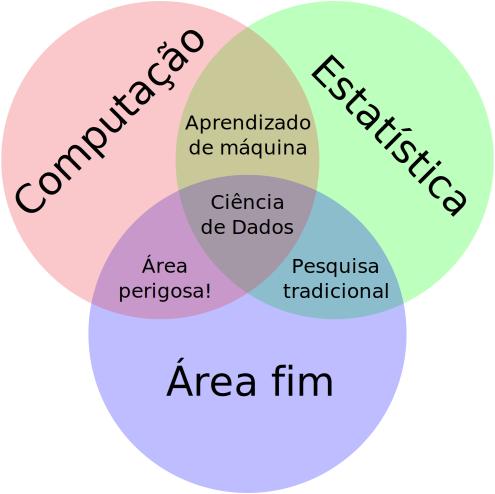
\includegraphics{ciencia-de-dados-diagrama-venn}
\caption{Diagrama de Venn mostrando as habilidades necessárias para um
cientista de dados}
\label{fig:ciencia-de-dados-venn}
\end{figure}

Com as técnicas da ciência de dados, podemos responder perguntas como ``Qual a
melhor rota para chegar até meu trabalho?'', ``Vai chover hoje?'', ``Quais são
minhas chances de desenvolver câncer nos próximos 10 anos?''. Neste trabalho,
estamos interessados nas técnicas de desenvolvimento de modelos preditivos que,
baseados nos dados e conhecimento que temos do assunto, determinam a
probabilidade de um resultado.

\subsection{Modelos preditivos}

\citeonline{Geisser1993} define modelagem preditiva como sendo ``o processo
pelo qual um modelo é criado ou escolhido para tentar melhor prever a
probabilidade de um resultado''. Já \citeonline{Kuhn2013} definem como ``o
processo de desenvolvimento de uma ferramenta ou modelo matemático que gere uma
previsão precisa''.

Modelos preditivos fazem parte do dia-a-dia da sociedade atual. O Google os
utiliza para interpretar o que seus usuários estão buscando; o Netflix usa para
recomendar filmes; corretoras de valores usam para definir que ações comprar ou
vender; seguradoras usam para definir qual o risco e, consequentemente, o preço
do seguro de um carro, entre outros \cite{Levy2010}.

Existem duas principais categorias de problemas que podem ser resolvidos por
modelos preditivos: regressão e classificação. A diferença entre eles está no
tipo de resposta que queremos prever, se é contínua ou categórica, o que
influencia nos tipos de modelos que podem ser usados e na forma de avaliá-los.
Por exemplo, ao analisarmos modelos que preveem o preço de um imóvel a partir
da sua área, buscamos o que chegue mais próximo do valor real\footnote{Esta é
uma simplificação. Existem diversas outras características a serem analisadas
ao escolher um modelo, como facilidade de interpretação, velocidade de
execução, entre outras. Aqui consideramos que a única diferença entre os
modelos seja o resultado previsto.}. Já ao avaliar modelos que classifiquem
imagens dos dígitos 0 a 9, só nos interessamos na classificação correta; dois
modelos que identifiquem a imagem do número 1 como sendo do número 3 e 8 estão
igualmente errados. O que classificou como 3 não está ``menos errado'' do que o
que classificou como 8 \cite{Kuhn2013,Zumel2014}. O foco deste trabalho é em
classificação. A seguir, apresentarei os modelos utilizados.

\subsubsection{glm}
Foo bar

\subsubsection{SVM}
Foo bar

\subsubsection{gbm}
Foo bar

\subsubsection{NB}
Foo bar

\subsubsection{RF}
Foo bar

\subsubsection{C5.0}
Foo bar

\subsection{Avaliando performance em modelos de classificação}
\label{cap:fundamentacao:avaliando-modelos-de-classificacao}

\nocite{Ng2012}

Uma das formas mais comuns de descrever a perfomance de um modelo de
classificação é através de uma ``matriz de confusão''. A tabela
\ref{table:exemplo-matriz-de-confusao} mostra um exemplo de matriz de confusão
com duas categorias: ``positivo'' e ``negativo''. Na diagonal principal estão
os valores classificados corretamente, e fora dela estão os erros. Dessa matriz
podemos extrair diversas métricas, como:

\begin{table}
\centering
\begin{tabular}{c c c}
  Previsto & \multicolumn{2}{c}{Observado} \\  \cline{2-3}
  & \multicolumn{1}{|c}{Positivo} & \multicolumn{1}{c|}{Negativo} \\
  \hline
  \multicolumn{1}{|c|}{Positivo} & Verdadeiro positivo (VP) & \multicolumn{1}{c|}{Falso positivo (FP)} \\
  \multicolumn{1}{|c|}{Negativo} & Falso negativo (FN) & \multicolumn{1}{c|}{Verdadeiro negativo (VN)} \\
  \hline
\end{tabular}
\caption{Matriz de confusão para um problema com duas classes: ``positivo'' e
``negativo''.}
\label{table:exemplo-matriz-de-confusao}
\end{table}

\begin{description}
\item[Número de amostras positivas]
\begin{equation}
\label{eq:positive-rate}
P = VP + FN
\end{equation}
\item[Número de amostras negativas]
\begin{equation}
\label{eq:negative-rate}
N = VN + FP
\end{equation}
\item[Acurácia] Proporção de predições corretas
\begin{equation}
\label{eq:accuracy}
ACC = \frac{VP + VN}{P + N}
\end{equation}
\item[Sensibilidade] Proporção de elementos da classe positiva classificados
corretamente em relação ao total de elementos positivos
\begin{equation}
\label{eq:sensitivity}
SENS = \frac{VP}{VP + FN}
\end{equation}
\item[Especificidade] Proporção de elementos da classe negativa classificados
corretamente em relação ao total de elementos negativos
\begin{equation}
\label{eq:specificity}
ESPEC = \frac{VN}{FP + VN}
\end{equation}
\end{description}

Dessas métricas, a com interpretação mais simples é a acurácia (equação
\ref{eq:accuracy}), que mede o percentual de predições corretas. Entretanto,
ela tem algumas limitações. Primeiramente, ela não leva em consideração o tipo
do erro. Em diversos problemas, o custo de um falso positivo é diferente do de
um falso negativo. Por exemplo, num sistema de classificação de spam, é
preferível que o usuário veja uma propaganda (falso negativo) do que deixe de
receber um e-mail importante (falso positivo). Além disso, ela também não
considera a frequência natural de cada classe. Se, por exemplo, 90\% dos
e-mails que eu receba não sejam spam, um modelo que simplesmente classifique
todo e-mail como não sendo spam terá 90\% de acurácia \cite{Kuhn2013}.

O \emph{Kappa} é uma métrica que leva em consideração as proporções das
classes. Ela pode assumir valores entre -1 e 1, sendo que 1 indica que todas as
predições foram corretas, -1 indica que todas foram erradas, e 0 que o modelo
tem uma performance igual a um aleatório. A equação \ref{eq:kappa} mostra como
calculá-la, onde $ACC$ é a acurácia observada e $ACC_{esperada}$ é a acurácia
esperada \cite{Cohen1960}.

\begin{equation}
\label{eq:kappa}
Kappa = \frac{ACC - ACC_{esperada}}{1 - ACC_{esperada}}
\end{equation}

Em geral, o resultado do uso de modelos de classificação é a probabilidade de
pertencimento a cada categoria. Por exemplo, um modelo pode, ao analisar um
e-mail, determinar que ele tem 75\% de chances de ser spam e, consequentemente,
25\% de chances de não ser. Para transformar essa probabilidade em uma
categoria define-se um ponto de corte \cite{Kuhn2013}.

Grande parte das ferramentas usa 50\% por padrão, que geralmente é uma escolha
interessante caso o custo de um falso positivo e falso negativo seja o mesmo e
as categorias sejam balanceadas. Caso contrário, é recomendável testar outros
valores. Uma ferramenta para analisar a sensibilidade e especificidade de um
modelo usando diferentes pontos de corte é a curva \gls{ROC}
\cite{Altman1994,Brown2006,Fawcett2006}.

A figura \ref{fig:exemplo-roc} mostra um exemplo de uma curva \gls{ROC} com os
valores discriminados em dois pontos: 0,5 e 0,614. A partir desse gráfico,
percebemos a troca entre sensibilidade e especificidade (quanto maior um, menor
o outro), e podemos escolher o melhor ponto de corte para o modelo em questão
levando em consideração nossos objetivos.

\begin{knitrout}
\definecolor{shadecolor}{rgb}{0.969, 0.969, 0.969}\color{fgcolor}\begin{figure}
\includegraphics[width=\maxwidth]{figure/tmp/exemplo-roc-1} \caption[Curva ROC de um modelo mostrando a área sob a curva (AUC) e dois pontos de corte]{Curva ROC de um modelo mostrando a área sob a curva (AUC) e dois pontos de corte: 0,5, o mais comum, e 0,614, o mais próximo do canto superior esquerdo.}\label{fig:exemplo-roc}
\end{figure}


\end{knitrout}

Além de auxiliar na escolha do ponto de corte, a curva \gls{ROC} também pode
ser usada para avaliar e comparar modelos desenhando-os num mesmo gráfico ou
comparando a área sob suas curvas (\acrshort{AUC}). O modelo na figura
\ref{fig:exemplo-roc} possui \acrshort{AUC} 0,787. Quanto mais próximo a curva está
do canto superior esquerdo, maior é seu \acrshort{AUC} e, em geral, maior é sua
performance.  O modelo perfeito tem \acrshort{AUC} 1, já um modelo aleatório
tem \acrshort{AUC} 0,5 e segue na diagonal do gráfico. O que caracteriza é um
\acrshort{AUC} bom ou ruim varia de caso a caso, mas \citeonline{HosmerJr2013}
definiram uma regra geral para avaliação descrita na tabela
\ref{table:valores-auc}.

\begin{table}
\centering
\begin{tabular}{c l}
  \acrshort{AUC} & \multicolumn{1}{c}{Valor} \\
  \hline
  0,5 & Não há discriminação \\
  Entre 0,7 e 0,8 & Discriminação aceitável \\
  Entre 0,8 e 0,9 & Discriminação excelente \\
  Acima de 0,9 & Discriminação excepcional \\
\end{tabular}
\caption{Regra geral para avaliação da \glsfirst{AUC} de \citeonline{HosmerJr2013}.}
\label{table:valores-auc}
\end{table}

\section{Teoria espacial do voto}
\label{cap:fundamentacao:teoria-espacial-do-voto}



É comum usar conceitos espaciais para identificar o posicionamento de
atores políticos. Por exemplo, dizemos que um deputado é de esquerda, enquanto
outro é de direita. A teoria espacial do voto é uma formalização dessas ideias.
Ela parte do pressuposto que as preferências individuais e as políticas podem
ser interpretadas como pontos em um espaço euclidiano. Um parlamentar então
votaria na política mais próxima da sua preferência, chamada de ponto ideal
\cite{Leoni2002}.

As dimensões desse espaço correspondem às áreas temáticas relevantes para os
atores, que podem ser muitas. Por exemplo, proteção do meio-ambiente, comércio
exterior, distribuição de renda, etc.

Considere um exemplo onde 5 parlamentares votam em um
projeto de Lei que propõe a redução da maioridade penal de
18 para 16 anos. Suponha
que cada um tem uma única preferência (\emph{single-peakedness}), que é o seu
ponto ideal, e vota sinceramente de acordo com ela, e que suas preferências são
simétricas. Isto é, dado duas escolhas a uma mesma distância do ponto ideal de
um parlamentar, ele será indiferente a qualquer uma delas.

Graficamente, temos a figura \ref{fig:modelo-espacial-votacao}, onde as curvas
representam as preferências dos legisladores sobre o assunto dessa votação, com
a altura representando a intensidade da preferência. Os pontos ideias estão nos
picos de cada curva. Há também três linhas, a azul representando o resultado de
um voto ``sim'', a vermelha o de um voto ``não'' (isto é, o \emph{status quo}),
e a preta representa a ``linha de corte'' dessa votação. As linhas de corte
passam pelo ponto médio entre as duas alternativas em votação, separando os
parlamentares que deverão votar sim dos que votarão não. Nesse exemplo, as
escolhas são entre uma maioridade penal de 16 ou
18, logo a linha de corte passa em $\frac{16 +
18}{2}$, ou seja, $17$. Caso o ponto ideal de um parlamentar esteja sobre essa
linha, ele é indiferente às alternativas.

% FIXME: Esse gráfico não funciona em preto e branco
\begin{knitrout}
\definecolor{shadecolor}{rgb}{0.969, 0.969, 0.969}\color{fgcolor}\begin{figure}
\includegraphics[width=\maxwidth]{figure/tmp/modelo-espacial-votacao-1} \caption[Preferências de 5 deputados na votação sobre a redução da maioridade penal de 18 para 16 anos]{Preferências de 5 deputados na votação sobre a redução da maioridade penal de 18 para 16 anos.  Parlamentares a esquerda da linha de corte nos 17 anos votam sim, e os a direita votam não. O deputado com preferência sobre a linha de corte é indiferente às duas opções. Neste exemplo, é ele quem desempata a votação.}\label{fig:modelo-espacial-votacao}
\end{figure}


\end{knitrout}

Há diversos modelos criados para estimar esses valores, como o NOMINATE,
W-NOMINATE, DW-NOMINATE, que são paramétricos; o Optimal Classification, que é
não-paramétrico, e; modelos baseados em estatística Bayesiana, como o IDEAL.
Nosso foco neste trabalho é no W-NOMINATE.
\cite{Poole1985,Poole2000,Poole2005,Jackman2000,Clinton2004}

O W-NOMINATE faz parte da família de modelos NOMINATE desenvolvidos por
\citeonline{Poole1985}. Eles são baseados no modelo de utilidade aleatória de
\citeonline{McFadden1976}, que define que a utilidade para um legislador em
votar de certa forma é formada por dois componentes: um determinístico e outro
estocástico (erro). Sendo $s$ o número de votações indexadas por $k = 1, ...,
s$; $p$ o número de legisladores indexados por $i = 1, ..., p$, e; $q$ o número
de votações indexados por $j = 1, ..., q$, a utilidade para o legislador $i$ da
consequência política do resultado ``sim'' da votação $j$ é definida como:

\begin{equation}
\label{eq:random-utility}
 U_{ijy} = u_{ijy} + \epsilon_{ijy}
\end{equation}

onde $u_{ijy}$ é a parte determinística e $\epsilon_{ijy}$ é a parte
estocástica da função utilidade $U_{ijy}$. Se não houver erro, o legislador vota sim se
$U_{ijy} > U_{ijn}$ e não se $U_{ijy} < U_{ijn}$, onde $y$ e $n$ representam as
consequências de um voto sim ou não, respectivamente. Caso $U_{ijy} = U_{ijn}$,
ele é indiferente ao resultado. Com o erro, a diferença entre as utilidades é:

\begin{equation}
U_{ijy} - U_{ijn} = u_{ijy} - u_{ijn} + \epsilon_{ijy} - \epsilon_{ijn}
\end{equation}

logo, um legislador vota sim se:

\begin{equation}
u_{ijy} - u_{ijn} > \epsilon_{ijy} - \epsilon_{ijn}
\end{equation}

ou seja, se a diferença das suas utilidades for maior que a diferença dos
erros. No W-NOMINATE, considera-se que a parte determinística $u_{ijy}$ segue a
distribuição normal, com os valores concentrados ao redor do ponto ideal do
legislador, e rapidamente tendendo a zero ao se afastar para ambos os lados.
Com isso, a equação \ref{eq:random-utility} se torna:

\begin{equation}
  U_{ijy} = \beta \exp^{\left( - \frac{1}{2} \sum\limits_{k=1}^s w_k^2 d_{ijky}^2 \right)} + \epsilon_{ijn}
\end{equation}

onde $\beta$ é uma constante que define o peso da parte determinística na
equação; $w_k$ é o peso da dimensão $k$, e; $d_{ijky}^2$ é a distância ao
quadrado na dimensão $k$ do legislador $i$ ($X_{ik}$) da consequência do
resultado sim da votação $j$ ($O_{jky}$):

\begin{equation}
d_{ijky}^2 = \left(X_{ik} - O_{jky}\right)^2
\end{equation}

O método então estima os valores de $O_{jky}$, $O_{jkn}$, $X_{ik}$, $\beta$ e
$w_k$.

% FIXME: Concluir

\subsection{Comparando pontos ideais ao longo do tempo}
\label{cap:fundamentacao:comparando-pontos-ideais-no-tempo}

O principal desafio em comparar mudanças nos pontos ideais ao longo do tempo é
distinguir alterações causadas por mudanças na agenda legislativa das causadas
por mudanças no posicionamento dos parlamentares \cite{Bailey2007}. Em outras
palavras, se o ponto ideal de um deputado federal passa de 0.3 para -0.2 de um ano
para o outro, como descobrir se isso representa uma mudança real de
posicionamento ou é somente reflexo da diferença na agenda legislativa dos dois
períodos?

Segundo \citeonline{Shor2010}, todos os esforços para resolver esse problema
usam ``pontes'', que podem ser parlamentares cujo posicionamento assume-se ter
se mantido estável durante o período de interesse, ou projetos de Lei que
foram votados em mais de um momento (nas duas casas legislativas em um sistema
bicameral, por exemplo). O primeiro é mais usado para comparar as mudanças dos
posicionamentos dos parlamentares, enquanto o segundo permite unir pessoas que
não votaram juntas em um mesmo mapa espacial\footnote{Por exemplo,
\citeonline{Shor2010} colocam todos os legisladores de 11 estados americanos e
do congresso federal em um período que varia entre 7 e 15 anos, dependendo do
estado, em um mesmo mapa espacial.}. \citeonline{Poole2005} propõe duas formas
para estimar pontos ideais usando pontes.

Na primeira forma, batizada de \emph{pooled scaling} por \citeonline{Shor2010},
dividimos os votos dos parlamentares que queremos mensurar em dois
parlamentares ``virtuais'', um com os votos antes e outro com os votos depois
da data de interesse. Unimos esses parlamentares virtuais com os
parlamentares-ponte, que possuem um registro único, em uma tabela individual e
executamos o algoritmo de estimação dos pontos ideais. Ao final, teremos dois
pontos para cada parlamentar de interesse e um ponto para os pontes. Na
segunda forma, que \citeonline{Shor2010} chamam de \emph{linear mapping},
estimamos os pontos ideias separadamente em cada período e os conectamos usando
uma regressão entre os conjuntos de pontos dos parlamentares-ponte. Ambas
formas devem gerar resultados similares, mas a segunda é computacionalmente
mais simples, o que pode ser essencial, dependendo da quantidade de
parlamentares e votações e votos em estudo.

\citeonline{Poole2005} ainda descreve uma terceira forma, similar a
\emph{pooled scaling} descrita acima, que usa para testar se os senadores
norte-americanos mudam de comportamento nos últimos dois anos de seus mandatos,
antes de concorrer à reeleição. Neste caso, ele quer calcular a mudança de
comportamento de todos os legisladores em dois momentos numa mesma legislatura.
Se usássemos o \emph{pooled scaling} diretamente, precisaríamos escolher alguns
parlamentares como pontes que, por definição, não teriam mudado de
comportamento. Ao invés disso, ele segue o seguinte processo:

\begin{enumerate}
  \item Para cada parlamentar, faça:
    \begin{enumerate}
      \item Transforme-o em dois parlamentares ``virtuais'', um com o conjunto
de votos antes, e outro com os depois da data de interesse. Os outros
parlamentares não são modificados;
      \item Calcule os pontos ideias;
      \item Guarde os resultados dos dois parlamentares ``virtuais''. A
diferença entre suas posições representa a mudança de comportamento do
parlamentar.
    \end{enumerate}
  \item Calcule medidas de incerteza para as estimativas.
\end{enumerate}

Ao final, ele tem dois pontos para cada senador: um representando sua posição
nos primeiros 4, e o outro nos últimos 2 anos da legislatura. Note que, como as
matrizes de votações usadas para gerar os mapas espaciais são diferentes, eles
não são estritamente comparáveis. Apesar disso, \citeonline{Poole2005}
argumenta que como elas possuem o mesmo conjunto de votos, com a única
diferença de que um dos parlamentares foi dividido em dois, ele considera ser
seguro compará-las.

\section{Processo legislativo}
\label{cap:fundamentacao:processo-legislativo}

Na esfera federal, o Poder Legislativo é exercido pelo Congresso Nacional, que
é composto por duas casas legislativas, constituindo um sistema bicameral. Essas
casas são a Câmara dos Deputados, que reúne os deputados federais,
representantes do povo, e o Senado Federal, que reúne os senadores,
representantes dos estados e Distrito Federal. Nas outras esferas (estadual,
distrital e municipal), o Poder Legislativo é unicameral.

As funções do Poder Legislativo se dividem em típicas e atípicas. Como típicas,
temos legislar \cite[arts. 48, 49, 51 e 52]{CF1988} e fiscalizar as entidades da
administração direta e indireta \cite[art. 70]{CF1988}. As funções atípicas são
administrar (por exemplo, seu quadro de servidores internos), e julgar (por
exemplo, crimes de responsabilidade do presidente da República). Além dessas,
\citeonline[p. 26]{Carneiro2013} mencionam que, como representantes do povo e da
nação, cabe ao Legislativo ``(...) debater temas importantes o que, muitas
vezes, não necessariamente resulta na inserção de uma nova norma no ordenamento
jurídico ou em uma fiscalização de determinada entidade ou agente público, o
que denota atuação inerente ao exercício da atividade parlamentar.''

O Senado Federal, também chamado de Casa Alta, é composto por 81 senadores, 3
por Estado e Distrito Federal. Os senadores têm mandato de 8 anos e são eleitos
pelo sistema majoritário\footnote{No sistema majoritário, o candidato mais
votado é eleito. Nos anos em que são eleitos 2 senadores, os dois candidatos
mais votados serão eleitos. Ele pressupõe um (ou dois) único candidatos por
partido. É o mesmo sistema usado nas eleições para os chefes do Poder Executivo
(presidente da República, governadores e prefeitos). Com exceção da eleição de
senadores e prefeitos em cidades com menos de 200 mil habitantes, onde há um
único turno, as eleições ocorrem em dois turnos. \cite{Carneiro2013}}. A
renovação da casa é parcial, modificando $\frac{1}{3}$ e $\frac{2}{3}$ dos
senadores alternadamente de 4 em 4 anos.

A Câmara dos Deputados, também chamada de Casa Baixa ou Casa do Povo, é
composta por 513 deputados federais, cujo papel é representar o povo. Cada
Estado ou Distrito Federal elege entre 8 e 70 deputados, proporcionalmente à
sua população. Os deputados têm mandato de 4 anos, eleitos pelo sistema
proporcional\footnote{No sistema proporcional os partidos registram vários
candidatos para o mesmo cargo. Os votos recebidos por cada candidato são
direcionados ao partido, que precisa atingir uma quantidade mínima de votos
(chamado quociente eleitoral) para eleger ao menos um de seus candidatos. Nesse
sistema, um candidato com menos votos pode se eleger, enquanto outro com mais
votos não se elegeu, dependendo dos seus partidos de filiação.
\cite{Carneiro2013,Bramatti2014}}. Diferente do Senado Federal, a renovação é
total de 4 em 4 anos.

O processo legislativo é classificado em ordinário, sumário e especial. O
primeiro se refere a elaboração de leis ordinárias, o sumário se diferencia por
apresentar prazo máximo para apreciação \cite[art. 64]{CF1988}, e o especial se
refere às outras normas jurídicas (e.x.: emendas constitucionais, medidas
provisórias, etc.). De acordo com \citeonline{Carneiro2013}, o processo
legislativo ordinário engloba três fases: 

\begin{description}
\item[Introdutória ou de iniciativa] \hfill \\
É onde se inicia o processo legislativo\footnote{O artigo 61 da Constituição
Federal define quem pode iniciar o processo legislativo. Exceto quando iniciado
por um Senador, o processo comeca com a Câmara dos Deputados como Casa
Iniciadora e, consequentemente, o Senado Federal como Casa Revisora.}, com o
projeto entrando em uma das Casas legislativas, denominada Casa iniciadora. Com
exceção dos projetos iniciados por Senadores, a Casa iniciadora é a Câmara dos
Deputados.

\item[Constitutiva] \hfill \\
A Casa iniciadora discutirá o projeto e poderá rejeitá-lo, enviando-o para o
arquivo, ou aprová-lo integralmente ou com emendas, caso em que passará para a
Casa revisora.

Igualmente, a Casa revisora poderá rejeitar o projeto e encaminhá-lo para o
arquivo, aprová-lo com emendas e devolvê-lo à Casa iniciadora para análise das
emendas sugeridas, ou aprová-lo integralmente e enviá-lo para sanção ou veto do
presidente. O projeto só passa para o presidente quando ambas as casas o
aprovam integralmente.

Uma vez o projeto estando com o presidente, ele poderá sancioná-lo e enviá-lo
para promulgação e publicação, ou vetá-lo parcial ou integralmente. Caso haja
um veto, ele será apreciado pelo Congresso Nacional dentro de trinta dias
corridos do seu recebimento, só podendo ser rejeitado pelo voto da maioria
absoluta dos deputados federais e senadores. Caso esse prazo se esgote, ele
será incluído na Ordem do Dia da próxima sessão do Congresso Nacional, se
sobrepondo às demais proposições até ser votado.

\item[Complementar] \hfill \\
É composta pela promulgação, instrumento do Poder Legislativo similar à
sanção do Poder Executivo, que atesta a existência da lei, e a subsequente
publicação no Diário Oficial da União. A lei entrará em vigor em 45 dias após
sua publicação ou em outra data definida nela própria. O intervalo entre sua
publicação e a entrada em vigor é conhecido como \emph{vacatio legis}.
\end{description}

Em linhas gerais, o projeto é iniciado em uma das casas legislativas
(normalmente a Câmara), que passa a ser conhecida como Casa Iniciadora. Ele é
discutido e, caso aprovado, passa para a outra casa legislativa, chamada de
Casa Revisora, que pode aceitá-lo integralmente (o que o faz seguir para sanção
ou veto pelo presidente da República); aceitá-lo com emendas e devolvê-lo à
Casa Iniciadora para apreciação das emendas sugeridas, ou; rejeitá-lo e
encaminhá-lo ao arquivo. Caso o presidente vete parcial ou integralmente o
projeto, o Congresso Nacional apreciará o veto, podendo mantê-lo e arquivar o
projeto, ou rejeitá-lo (por maioria absoluta) e devolvê-lo ao presidente para
promulgação \cite{Carneiro2013}.

Existem dois tipos de votação: ostensiva e secreta. A votação ostensiva é
utilizada nas proposições em geral, e é a regra na Câmara dos Deputados. Ela
pode ocorrer pelos processos simbólico ou nominal. No processo simbólico, o
presidente da casa, ao anunciar a votação, convida os deputados a favor da
matéria a permanecerem sentados, devendo os contrários manifestarem-se
(normalmente levandando um braço). No processo nominal, os parlamentares votam
usando um meio eletrônico ou, em caso de falha, por chamada nominal
\cite{Carneiro2013}.

Na Câmara dos Deputados, o processo nominal é utilizado nos casos em que seja
exigido quórum especial de votação (como nas emendas constitucionais); por
deliberação do Plenário, a requerimento de qualquer deputado, e; quando houve
pedido de verificação de votação por 6\% dos membros da Casa (31 deputados), ou
líder que represente esse número \cite[art. 186]{RICD2015}. No geral, as
votações nominais compreendem o subconjunto de decisões mais importantes e
polêmicas \cite{Figueiredo2001}.

\section{Considerações Finais}

O objetivo deste capítulo foi fornecer um conjunto mínimo de conhecimento
necessário para a compreensão do restante deste trabalho. Para isso, foram
descritos o processo de desenvolvimento e avaliação de modelos preditivos,
focando em modelos de classificação. Em seguida, foi explicada brevemente a
teoria espacial do voto, em especial a técnica W-NOMINATE. Por fim, o processo
legislativo brasileiro a nível federal foi descrito, com ênfase nos tipos de
votação.

No próximo capítulo, serão apresentados alguns trabalhos relacionados aos temas
desta dissertação, analisando suas metodologias e resultados em comparação com
o deste trabalho.
\chapter{Trabalhos Relacionados}\label{cap:trabalhos-relacionados}


\section{Análise do comportamento parlamentar}
\label{cap:trabalhos-relacionados:analise-comportamento}

No final da década de 80 e na de 90, diversos autores viam o sistema político
brasileiro como sendo altamente instável, com um Poder Executivo fraco,
obrigado a negociar com cada parlamentar individualmente para executar seu
plano de governo. Os parlamentares, preocupados somente com seus interesses
individuais e regionalistas, seriam indisciplinados, levando a
ingovernabilidade do país
\cite{Abranches1988,Lamounier1994,Mainwaring2001,Ames2003}.

Contrários a esse diagnóstico, \citeonline{Limongi1995} descreveram um cenário
muito diferente. O Executivo, por ter domínio sobre a agenda legislativa,
seria capaz de executar seu plano de governo negociando diretamente com os partidos
políticos, que seriam capazes de disciplinar seus parlamentares a votar
conforme suas indicações. Esse diagnóstico foi feito a partir da análise das
votações nominais na Câmara dos Deputados no período de 1989 a 1994. Nessa
análise, os autores calcularam a coesão interna de cada partido, usando o
\gls{IR}\footnote{O \glsfirst{IR} varia de 0 a 100, e é calculado subtraindo a
proporção dos votos minoritários dos majoritários. Ele é 0 quando o partido
está dividido, com metade votando sim e a outra metade votando não, e é 100
quando todos os parlamentares votam da mesma forma \cite{Rice1924}.}. Todos os
partidos apresentaram níveis de coesão relativamente altos, com o menos coeso,
o PDS, atingindo um \gls{IR} 75,70, e o mais coeso, o PT, com \gls{IR} 95,96.

Essas duas correntes foram tão distintas que \citeonline{Power2010} as dividiu
em ``pessimistas'' e ``otimistas''.

Figueiredo e Limongi continuaram analisando dados relacionados ao mesmo tempo,
focando em períodos e características distintos, que confirmaram o prognóstico.
A coletânea desses artigos gerou o livro ``Executivo e Legislativo na nova
ordem constitucional'' \cite{Figueiredo2001}.

Também usando métricas de coesão, \citeonline{Cheibub2009} concluem que o
Congresso brasileiro, ao contrário do previsto pelos pessimistas, é altamente
centralizado, com partidos e seus líderes capazes de disciplinar seus
parlamentares, evitando que estes ajam somente em busca de benefícios para si
mesmo e seus redutos eleitorais.

Além de cientistas políticos, jornalistas também têm usado técnicas semelhantes
para análise das votações. O Grupo Estado, dono do jornal Estado de São Paulo
(o Estadão), lançou em maio de 2012 a ferramenta Basômetro\footnote{Disponível
em \url{http://estadaodados.com/basometro/}.}, um site interativo que permite a
análise de como os parlamentares, individualmente e agregados por partido,
votaram, com dados a partir do primeiro governo de Lula em 2003. Além da
análise de cada votação, o Basômetro também calcula a taxa de
governismo\footnote{A taxa de governismo é calculada como o percentual de vezes
que os parlamentares votaram de acordo com a posição do governo.} dos partidos
e parlamentares, mostrando suas flutuações em cada mês \cite{Estadao2012}.

\citeonline{Dantas2014} organizaram uma coletânea de artigos escritos baseados
em análises feitas com o Basômetro gerando o livro ``Análise política \&
jornalismo de dados''.

Apesar de serem de interpretação e cálculo mais simples, métricas de coesão têm
alguns problemas. Em primeiro lugar, pela distância entre valores não ser
uniforme (por exemplo, a distância entre 40\% e 50\% não é necessariamente
igual a entre 50\% e 60\%), eles só ordenam os parlamentares. Há também um
baixo valor de números possíveis. Em $p$ votações, há $p + 1$ valores
possíveis. Por exemplo, em 3 votações, os parlamentares só podem assumir os
valores 0\%, 33\%, 66\% e 100\%. Por fim, o índice é calculado em relação a
algum ponto específico. Por exemplo, a taxa de governismo é calculada com base
no voto do governo, que normalmente é definido pela indicação ou voto do líder
do governo. Assim, ninguém pode ser mais governista do que o próprio líder, o
que é um pressuposto que precisa ser testado
\cite{Poole2005,McCarty2011,Izumi2013}. Para evitar essas limitações, diversos
autores usam modelos espaciais de votação (ver Seção
\ref{cap:fundamentacao:teoria-espacial-do-voto}).

No Brasil, o primeiro autor a usar esses modelos foi \citeonline{Leoni2002},
que analisou o posicionamento dos deputados federais entre 1991 e 1998 usando o
W-NOMINATE. \citeonline{Desposato2005b} usou o mesmo método para analisar o
efeito da mudança partidária no comportamento dos parlamentares.
\citeonline{Zucco2009} também usa o W-NOMINATE, dessa vez para entender os
fatores que influenciam o comportamento dos parlamentares, encontrando
que a ideologia não explica completamente seus comportamentos, e indicativos
que o presidente da República é um importante influenciador, especialmente
através da distribuição de cargos e recursos.

\citeonline{Freitas2012} analisam o significado da primeira dimensão, estimada
usando W-NOMINATE, na Câmara dos Deputados e no Senado Federal, concluindo que
ela está ligada ao conflito governo e oposição. \citeonline{Izumi2013} repete
essa análise no Senado Federal usando outro modelo, o \emph{Optimal
Classification}, chegando a mesma conclusão.

Além de técnicas específicas para gerar mapas espaciais de votação, alguns
autores usaram técnicas de redução de dimensionalidade mais gerais.
\citeonline{Trento2013} analisaram os dados da Câmara dos Deputados, Senado
Federal e Câmara Municipal de São Paulo usando \gls{ACP}\footnote{Do inglês,
\emph{Principal Component Analysis} (PCA).}, uma técnica estatística de redução
de dimensionalidade. Eles mapeiam um voto sim ou não nos valores 1 e 0, e
transformam o conjunto de votos dos parlamentares em pontos em um espaço
n-dimensional, onde cada dimensão representa uma votação. Como o número de
votações é alto, é difícil visualizar esses pontos. Assim, usam o \gls{ACP}
para colocar esses pontos em um espaço bidimensional, mantendo ao máximo suas
posições relativas. Dessa forma, quanto mais próximo estiverem dois
parlamentares (ou partidos), mais vezes eles votaram da mesma forma. O
resultado dessa pesquisa foi o Radar Parlamentar\footnote{Disponível em
\url{http://radarparlamentar.polignu.org}}, um site interativo no qual é
possível visualizar os diversos gráficos gerados, com as posições dos
legisladores e partidos a cada ano.

Usando uma técnica semelhante, a \gls{MCA}, \citeonline{Andrade2015} colocam os
deputados federais em um espaço bidimensional, mostrando aonde estaria o
presidente da Câmara dos Deputados, Eduardo Cunha (PMDB/RJ). Como ele não vota,
consideraram seu posicionamento como sendo igual ao do líder do PMDB na Câmara
no período. Eles também analisaram a similaridade dos deputados com o Eduardo
Cunha através do percentual de votos que deram iguais a ele, batizando essa
métrica de ``Cunhômetro''.

Apesar dessas técnicas estatísticas como a \gls{ACP} e \gls{MCA} serem
similares a técnicas como o W-NOMINATE, não encontramos trabalhos que validem
seu uso em dados de votação, o que pode dificultar a interpretação dos seus
resultados.

% FIXME: Citar o GovTrack.us e https://opengovdata.io/

\subsection{Análise da mudança de comportamento parlamentar}

O problema básico em comparar mudanças de comportamento ao longo do tempo é
distinguir alterações por causa de uma mudança de agenda das causadas por uma
real mudança das preferências dos parlamentares \cite{Bailey2007}. Em outras
palavras, se em um momento dois parlamentares votaram 90\% das vezes da mesma
forma, e em outro momento eles votaram 50\% das vezes, como definir se essa
mudança se deu porque eles mudaram seus posicionamentos, ou simplesmente porque
eles concordavam nas votações do primeiro momento, mas não nas do segundo?

Segundo \citeonline{Shor2010}, todos os esforços para resolver esse problema
usam ``pontes'', que são parlamentares que estiveram presentes em ambos
momentos e cujo posicionamento se assume ter se mantido estável. Podemos citar
como exemplos parlamentares que foram eleitos para mais de uma legislatura, ou
que mudaram de Casa (deputados federais que se tornam senadores). Projetos de
Lei também podem ser usados como ponte, caso eles tenham sido votados nas
instituições ou períodos de interesse.

No artigo, \citeonline{Shor2010} usam três tipos de pontes para colocar
parlamentares que serviram no nível estadual em ambas as casas\footnote{O
sistema legislativo norte-americano, ao contrário do brasileiro, é bicameral
tanto a nível federal quanto estadual (exceto o estado de Nebrasca, que só
possui um Senado estadual)}, federal em ambas as casas, e no tempo.
Parlamentares que serviram por múltiplas legislaturas tanto a nível estadual
quanto federal servem de ponte entre as legislaturas; legisladores que passam
da casa baixa para a casa alta (ou vice-versa) em nível estadual conectam as
respectivas casas, e; parlamentares que passam do nível estadual para atuar no
nível federal conectam o estado com o Congresso.

No Brasil, \citeonline{Leoni2002} analisa as posições dos deputados federais na
49\textordfeminine{} e 50\textordfeminine{} legislaturas não usando pontes, mas
sim a correlação de Pearson entre os pontos ideais. Ele encontrou correlações
altas, em torno de 0,80. Apesar disso, ele reconhece que uma limitação de seu
trabalho é que, nos períodos estudados, o governo sempre foi de direita, o que
poderia causar essa baixa mudança de pontos ideais. Além disso, como ele não
usou nenhuma técnica para diferenciar mudanças de comportamento de mudanças na
agenda legislativa (como as pontes), não é possível distinguir a razão desse
resultado com segurança.

\citeonline{Desposato2005b}, ao analisar o impacto das mudanças de partido no
comportamento dos parlamentares, usou o posicionamento dos legisladores que não
mudaram de partido como pontes. \citeonline{Izumi2013} faz uma pesquisa
semelhante, mas analisando a mudança de comportamento dos senadores que mudaram
de um partido dentro da coalizão governamental para um fora (ou vice-versa),
para entender o efeito da coalizão no comportamento dos parlamentares.

O Basômetro e o Radar Parlamentar não diferenciam mudanças de comportamento
reais das causadas por mudança da agenda legislativa
\cite{Estadao2012,Trento2013}.

Em geral, trabalhos que usam métricas de coesão interpretam as razões de
mudanças de comportamento usando métodos qualitativos, enquanto os que usam
pontos ideais usam métodos quantitativos.

\section{Aprendizagem de máquina na Ciência Política}
\label{ref:trabalhos-relacionados:data-science-polsci}

Os trabalhos encontrados que usam técnicas de aprendizagem de máquina no
âmbito da Ciência Política dividem-se em duas categorias: os que analisam
textos (como discursos) buscando entender seu conteúdo ou o posicionamento do
autor, e os que analisam projetos de lei tentando prever seus resultados.

Dos que fazem análise textual, \citeonline{Thomas2006} criaram um modelo que
classifica os discursos em debates sobre projetos de lei no congresso
estadunidense como sendo contrários ou favoráveis ao mesmo.
\citeonline{Quinn2006} criaram um modelo que extrai tópicos do texto de
discursos, validando-o nos dados do 105\textordmasculine{} ao
107\textordmasculine{} senado dos Estados Unidos. \citeonline{Yu2008}
determinam a filiação partidária dos parlamentares estadunidense a partir dos
seus discursos. \citeonline{Somasundaran2010} classificam autores de textos
publicados na Internet identificando seu posicionamento político a partir de
suas argumentações. Já \citeonline{Conover2011} fazem o mesmo com os usuários do
Twitter\footnote{Disponível em \url{http://twitter.com}.}, mas a partir da
frequência do uso de certas palavras.

Já na previsão do sucesso de projetos de lei, \citeonline{Gerrish2011} e
\citeonline{Goldblatt2012} desenvolveram modelos que acertaram mais de 90\% dos
resultados nos períodos estudados. \citeonline{Yano2012} fizeram uma análise
semelhante, mas focando em prever os projetos de lei que conseguirão passar das
discussões ocorridas em comissões e ser postos em votação.
\citeonline{Wang2012} preveem os resultados através de uma caminhada aleatória
em 3 grafos heterogêneos interconectados, sendo dois representando os
legisladores e um representando projetos de lei. Os legisladores estão
interligados caso tenham escrito ao menos um projeto juntos\footnote{Do inglês,
\emph{co-sponsorship}.}, e os projetos de lei interligados pela análise da
similaridade textual. Quando um legislador vota em um projeto de lei, um
vértice é criado entre seu nó e o do projeto. Ele criou dois grafos para os
legisladores como forma de criar dois tipos de ligação entre os legisladores e
os projetos de lei: uma para representar votos sim, e outra para votos não.

A empresa americana \citeonline{FiscalNote2015} desenvolve ferramentas para
monitoramento legislativo usando técnicas de ciência de dados. Uma delas, a
\emph{Prophecy}\footnote{Disponível em
\url{https://www.fiscalnote.com/prophecy}.} (do inglês, profecia), supostamente
prevê o resultado de projetos de lei com 94\% de acurácia. No Brasil, o
\gls{ELLO}, empresa ligada ao \gls{CEBRAP}, possui um produto similar.

\section{Considerações Finais}

Como visto na Seção \ref{cap:trabalhos-relacionados:analise-comportamento}, o
foco da literatura encontrada é na análise e interpretação do comportamento dos
parlamentares, seja usando métricas de coesão ou modelos espaciais de votação.
Na Seção \ref{ref:trabalhos-relacionados:data-science-polsci}, foram
apresentados trabalhos que aplicam técnicas de aprendizagem de máquina em temas
da ciência política, buscando descobrir o posicionamento de pessoas através dos
seus textos ou prever o resultado de votações.

Nesse levantamento bibliográfico, não foi encontrado nenhum autor que
desenvolva o objetivo deste trabalho: a detecção de mudanças de posicionamento
dos legisladores. O que parece ser mais próximo é a pesquisa feita pela empresa
americana \citeonline{FiscalNote2015} para o desenvolvimento do produto
\emph{Prophecy}, mas não foi possível analisar as semelhanças mais a fundo pois
o processo usado por eles não é divulgado.

Nesse sentido, considero a definição da metodologia para o desenvolvimento de
um modelo de detecção de mudança de posicionamento dos deputados federais
brasileiros como sendo o principal diferencial e contribuição deste trabalho.






\chapter{Desenvolvimento do modelo preditivo}\label{cap:desenvolvimento}

Neste capítulo apresentaremos o processo de criação do modelo preditivo,
partindo da coleta e preparação dos dados, onde serão estimadas as mudanças de
comportamento, passando pela análise dos dados visando definir os preditores
(variáveis independentes). Ao final, treinaremos 6 tipos de modelos diferentes,
escolhendo o final de acordo com a \glsfirst{AUC}.

\section{Coleta dos dados}



Os votos e votações foram extraídos diretamente do site da Câmara dos
Deputados através de sua \gls{API} \cite{CamaraDosDeputados2015}. Para
desenvolver o modelo preditivo, precisamos ter acesso a todos os dados na
máquina local. Entretanto, até a data de escrita deste trabalho, a \gls{API} da
Câmara só permitia consultas individuais, votação por votação, por isso
desenvolvi um programa\footnote{Disponível em:
\url{https://github.com/vitorbaptista/dados-abertos-camara.gov.br}} na
linguagem Python que, com o auxílio da biblioteca Scrapy, baixa todas as
votações \cite{Python276,Scrapy}. A tabela
\ref{table:estatisticas-legislaturas} mostra o número de deputados federais,
votos e votações por legislatura. Em média, temos 624
parlamentares e 332 votos em
478 votações a cada legislatura.

\begin{table}
\centering
\begin{knitrout}
\definecolor{shadecolor}{rgb}{0.969, 0.969, 0.969}\color{fgcolor}
\begin{tabular}{r|r|r|r}
\hline
Legislatura & Deputados Federais & Votações & Votos\\
\hline
50 & 631 & 468 & 178603\\
\hline
51 & 624 & 419 & 155737\\
\hline
52 & 614 & 451 & 134461\\
\hline
53 & 606 & 619 & 192879\\
\hline
54 & 644 & 432 & 131552\\
\hline
\end{tabular}


\end{knitrout}
\caption{Número de deputados federais e votações por legislatura}
\label{table:estatisticas-legislaturas}
\end{table}

% Coalizão
A lista das coalizões foi obtida através do banco de dados
legislativos do \gls{CEBRAP}. Ela contém a data de início e fim e a composição
partidária de cada coalizão. Como trabalhamos com os parlamentares
individualmente, gerei outra lista que contém todas as entradas e saídas dos
deputados federais na coalizão dentro de uma mesma legislatura. Por exemplo,
apesar do deputado Arlindo Chinaglia (PT/SP) passar de oposição a governo
em 2003 com a eleição de Lula, não consideramos isso uma mudança pois ela
ocorreu entre legislaturas. Já a saída de Romário (PSB/RJ) da coalizão quando
seu partido se tornou oposição em 2013 é considerada, pois ocorreu dentro de
uma mesma legislatura.

As coalizões são compostas pelos partidos que controlam ao menos um ministério.
Uma nova coalizão é formada em duas situações: i) na mudança de legislatura, e;
ii) na mudança do conjunto de partidos que controlam ministérios. Em outras
palavras, uma nova coalizão é formada quando um partido que não possuía nenhum
ministério passa a ter ao menos um, quando um partido que controlava algum
ministério passa a não ter nenhum, ou quando se inicia uma nova legislatura.
Esses critérios foram definidos por \citeonline{Figueiredo2007}, inspirada no
trabalho de \citeonline{Muller2000}.

\begin{knitrout}
\definecolor{shadecolor}{rgb}{0.969, 0.969, 0.969}\color{fgcolor}\begin{figure}
\includegraphics[width=\maxwidth]{figure/tmp/mudancas-mensais-de-coalizao-1} \caption[Número de deputados federais que mudaram de posicionamento, entrando ou saindo da coalizão entre a 50\textordfeminine{} e 54\textordfeminine{} legislaturas agrupados mês a mês]{Número de deputados federais que mudaram de posicionamento, entrando ou saindo da coalizão entre a 50\textordfeminine{} e 54\textordfeminine{} legislaturas agrupados mês a mês.}\label{fig:mudancas-mensais-de-coalizao}
\end{figure}


\end{knitrout}

A figura \ref{fig:mudancas-mensais-de-coalizao} mostra as
890 entradas e saídas da coalizão que ocorreram
durante o período de estudo, agrupadas mensalmente. Há meses que concentram
as mudanças de posicionamento, que serão melhor analisadas na seção
\ref{cap:desenvolvimento:aspectos-temporais}. A linha tracejada marca a data da Resolução
n\textordmasculine{} 22.610 do TSE, que em 24/10/2007
alterou o entendimento das regras de fidelidade partidária, tornando-as mais
restritas \cite{TSE2007}, o que aparentemente alterou os aspectos temporais das
mudanças de posicionamento.

\section{Preparação dos dados}

% Universo de votações

% FIXME: Confirmar uso da crase
O período de análise deste trabalho é composto pela 50\textordfeminine{},
51\textordfeminine{}, 52\textordfeminine{}, 53\textordfeminine{} e
54\textordfeminine{} legislaturas, compreendendo os 20 anos de 1995 até o
início de 2015, entre o primeiro mandato de Fernando Henrique Cardoso até o
final do primeiro mandato de Dilma Rousseff. As 48\textordfeminine{} e
49\textordfeminine{} legislaturas, iniciadas respectivamente em 1987 e 1991,
foram excluídas, pois, segundo \citeonline{Freitas2008}, elas ocorreram em um
período onde parlamentares ainda estavam se acomodando às novas regras advindas
da transição à democracia.

% Universo de parlamentares

A análise se restringe à Câmara dos Deputados por três razões: facilidade na
obtenção dos dados; maior número de parlamentares (513 contra 81 no Senado
Federal), e; por normalmente ser a casa iniciadora, mais votações ocorrem na
Câmara \cite{Vicente2012}.

A unidade de análise usada é o parlamentar, pois, apesar da literatura apontar o
papel fundamental dos partidos no comportamento dos parlamentares
\cite{Figueiredo2001,Santos2003,Freitas2008}, trabalhar com os dados
desagregados nos permite perceber movimentações como quando um parlamentar
deixa um partido governista para entrar em um de oposição (ou vice-versa).
Considerei todos os parlamentares que votaram ao menos uma vez na Câmara, por
isso o número é maior do que os 513 eleitos por legislatura.

% Universo de votos

Os deputados podem votar sim, não, nulo, branco, se abster ou obstruir
\cite{Carneiro2013}, mas o método W-NOMINATE usado neste trabalho só considera
votos sim ou não. Isso nos dá duas opções: mapear os outros tipos de votos como
sendo a favor ou contra (por exemplo, considerando abstenções como votos
contrários), ou ignorá-los. Para evitar possíveis problemas metodológicos ao
criar critérios desse tipo, desconsidero votos diferentes de sim ou não.

\subsection{Estimando a mudança de comportamento}
\label{cap:desenvolvimento:estimando-mudanca-comportamento}

Para estimar a mudança de comportamento, seguirei a metodologia de
\citeonline{Poole2005} descrita na seção
\ref{cap:fundamentacao:comparando-pontos-ideais-no-tempo} usando o modelo
W-NOMINATE \cite{Poole1985}. Esse modelo foi escolhido pois, apesar de
diversos outros modelos terem sido desenvolvidos nos 30 anos desde sua criação,
ele continua sendo um dos modelos mais usados \cite{Poole2011}, inclusive no
Brasil \cite{Leoni2002,Desposato2005b,Zucco2009,Freitas2012,Bernabel2015}.

Ao estimar os pontos ideais usando esse modelo, precisamos definir 5
parâmetros: número de dimensões; polaridade(s); critérios de inclusão de
parlamentares e votações; número de repetições para estimar o erro, e; período
de análise. Eles serão definidos nas próximas subseções.

\subsubsection{Número de dimensões}

\citeonline{Leoni2002} analisou o número de dimensões necessárias para explicar
o comportamento dos parlamentares na Câmara dos Deputados de 1991 a 1998.
\citeonline{Freitas2012} expandiram esse trabalho analisando não só a Câmara,
mas também o Senado Federal, usando os dados do período de 1988 a 2010.
\citeonline{Izumi2013} analisou o Senado de 1989 a 2010 usando outro modelo
espacial de votação, o \emph{Optimal Classification}. Exceto durante a
49\textordfeminine{} legislatura, onde tivemos dois presidentes (Collor e
Itamar Franco), todos concluíram que o congresso é predominantemente
unidimensional. Como essa legislatura não será analisada neste trabalho, usarei
uma única dimensão.

\subsubsection{Polaridade}

A polaridade define qual é a direção dos eixos das dimensões. No caso de uma
única dimensão, o parlamentar escolhido como polaridade será colocado nos
valores positivos. Idealmente, deve-se escolher um parlamentar que não tenha
mudado de posicionamento no período e que tenha participado do maior número de
votações. Como o PT é, historicamente, um dos partidos mais coesos do Brasil e
nunca mudou de posicionamento durante uma legislatura, sendo sempre oposição
até se tornar governo com a eleição de Lula em 2003, escolhi parlamentares
filiados a ele como polaridade.

O deputado José Genoíno foi usado nas 50\textordfeminine{},
51\textordfeminine{} e 53\textordfeminine{} legislaturas, Arlindo Chinaglia na
52\textordfeminine{} e Luiz Couto na 54\textordfeminine{}. Eles foram
escolhidos pois nunca trocaram de partido, ocuparam cargos de liderança e
participaram de um grande número de votações nas legislaturas em que foram
escolhidos.

\subsubsection{Critérios de inclusão de parlamentares e votações}
\label{cap:desenvolvimento:criterios-de-inclusao}

Incluímos parlamentares que participaram de no mínimo 20 votações cujo lado
minoritário foi responsável por 2,5\% ou mais dos votos. Esses são os critérios
padrão do W-NOMINATE, seguidos nos trabalhos de
\citeonline{Leoni2002,Zucco2009,Freitas2012}.

\subsubsection{Períodos de análise}
\label{cap:desenvolvimento:periodos-de-analise}

Na análise de uma mudança de comportamento, é preciso definir ao menos dois
períodos: um anterior e outro posterior a data de interesse. Por exemplo, para
analisar o efeito da saída do PSB da coalizão em outubro de 2013 no
comportamento dos parlamentares, poderíamos definir o período inicial como
sendo do início da legislatura até a data da saída do PSB, e o período final
como sendo da saída do PSB até o final da legislatura. Como o objetivo deste
trabalho não é analisar um período específico, mas criar um modelo que detecte
mudanças na coalizão, não basta definir um, mas sim um conjunto de
períodos.

Ao definir esses períodos é preciso levar em consideração diversos fatores.
Períodos muito curtos, por exemplo uma semana antes e uma semana depois, podem
sofrer com a falta de votações suficientes ou serem demasiadamente
influenciados por votações anômalas. Já períodos muito longos, como 5 anos
antes e 5 anos depois, dificultam a interpretação dos resultados pois podem
conter diversas mudanças de comportamento. No mínimo, precisamos de um período
que contenha votações suficientes de acordo com nossos critérios de inclusão
definidos na seção \ref{cap:desenvolvimento:criterios-de-inclusao}.

Baseado nisso, defini períodos de 12 meses dentro de uma mesma legislatura
divididos em duas partes de mesmo tamanho. Eles iniciam no primeiro dia de cada
mês, partindo de 01/Fev no primeiro ano da legislatura até o do último. Por
exemplo, na 54\textordfeminine{} legislatura, o primeiro período vai de
01/Fev/2011 até 01/Fev/2012 (dividido em 01/Ago/2011), e o último vai de
01/Fev/2014 até 01/Fev/2015. Existem 37 desses períodos por legislatura, 185
nas 5 legislaturas estudadas neste trabalho. A arbitrariedade dessa escolha é
uma limitação deste trabalho, que será melhor analisada na seção
\ref{cap:conclusao:limitacoes}.

\subsubsection{Estimativas de erro}

\citeonline{Poole2005} sugere, sem justificar esse número, repetir as
estimativas 101 vezes para calcular seu erro. Entretanto, o volume de dados que
estamos trabalhando invibializa esse número de repetições com os recursos
computacionais disponíveis para esta pesquisa\footnote{Por exemplo, usando um
núcleo de um processador AMD Opteron\texttrademark{} 6238 com 2,6 GHz o
processamento dos pontos ideais de um parlamentar em um período demora cerca de
1h45m. Considerando somente os 513 deputados eleitos por legislatura, o
cálculo de todos os 37 períodos levaria aproximadamente 18 meses. Todas as 5
legislaturas analisadas neste trabalho levariam mais de 7 anos. O cálculo é
facilmente paralelizável, diminuindo o tempo necessário de acordo com o número
de processadores, mas ainda assim não foi possível usar 101 repetições neste
trabalho.}. Por isto, escolhi fazer 10 repetições, o que diminuiu o tempo
necessário em cerca de 90\%.

\begin{table}
\centering
\begin{knitrout}
\definecolor{shadecolor}{rgb}{0.969, 0.969, 0.969}\color{fgcolor}
\begin{tabular}{r|r|r|r|l}
\hline
antes & antes.sd & depois & depois.sd & mudou\_posicionamento\\
\hline
0.55 & 0.02 & -0.40 & 0.03 & Sim\\
\hline
0.90 & 0.01 & 0.85 & 0.02 & Não\\
\hline
-0.30 & 0.01 & 0.40 & 0.01 & Sim\\
\hline
\end{tabular}


\end{knitrout}
\caption{Exemplo da tabela usada para treinar o algoritmo.}
\label{table:dataset-final}
\end{table}

\subsection{``Raio de influência'' de uma mudança de posicionamento}
\label{cap:desenvolvimento:raio-de-influencia}

Até esse momento, temos uma tabela onde cada linha representa um parlamentar em
um período, e nas colunas temos seus pontos ideais e as respectivas estimativas
de erro. Em outras palavras, temos nossas variáveis independentes, agora
precisamos determinar a variável dependente: se o parlamentar mudou de
posicionamento, entrando ou saindo da coalizão, ou se manteve como estava.

Para isso, precisamos definir qual o período antes de uma mudança de
posicionamento que o parlamentar começa a mudar de comportamento. Por exemplo,
considere que detectamos que um parlamentar que está fora da coalizão se
aproximou do governo entre o primeiro e o segundo semestre de 2011, mas só
entrou na coalizão em 2014. Devemos considerar que essa aproximação em 2011 foi
indício da sua entrada em 2014? E se ela tivesse ocorrido em 2012?  Em outras
palavras, precisamos definir qual o ``raio de influência'' de uma entrada ou
saída da coalizão.

Não há uma resposta única. Alguns parlamentares podem mudar de comportamento
anos antes de mudarem de posicionamento, enquanto outros podem não mudar em
momento algum. A hipótese fundamental deste trabalho é que eles mudam de
comportamento antes de mudar de posicionamento, caso contrário seria impossível
prever um a partir do outro. Formalmente, sendo $Data_{coaliz\tilde{a}o}$ a
data de entrada ou saída da coalizão, $Data_{inicial}$ e $Data_{final}$ as
datas iniciais e finais do período analisado, $Data_{m\acute{e}dia}$ a data que
divide o período analisado em dois, ``antes'' e ``depois'', e $P =
Data_{m\acute{e}dia} - Data_{inicial} = Data_{final} -
Data_{m\acute{e}dia}$ a distância da data inicial até a data média, que é igual
a da data média até a data final, então o período em que consideramos que uma
mudança de comportamento esteja relacionada a mudança de posicionamento
compreende $\left[Data_{m\acute{e}dia} - \frac{P}{2}, Data_{m\acute{e}dia} +
\frac{P}{2}\right]$. Precisamos definir $P$.

Para entender melhor, vejamos a figura \ref{fig:raio-de-influencia-coalizao}.
Nela são mostrados cinco períodos de análise de um parlamentar que mudou de
comportamento em $Data_{coaliz\tilde{a}o} - P$, representado pela mudança da
região azul para a verde, com o período de análise em cada momento representado
pela região escurecida entre $Data_{inicial}$ e $Data_{final}$. No primeiro
período, \ref{fig:raio-de-influencia-coalizao1}, a $Data_{final}$ é igual ao
momento de mudança de comportamento. Aqui, não consideramos que houve uma
mudança de posicionamento, pois o comportamento dentro desse período é
constante (região azul). Na figura \ref{fig:raio-de-influencia-coalizao2}, a
mudança de comportamento ocorre no ponto médio entre a $Data_{m\acute{e}dia}$ e
a $Data_{final}$. A partir daqui começamos a considerar que o parlamentar mudou
de posicionamento. Na figura \ref{fig:raio-de-influencia-coalizao3}, a
$Data_{final} = Data_{coaliz\tilde{a}o}$, e a $Data_{m\acute{e}dia}$ se iguala
a data da mudança de comportamento em $Data_{coaliz\tilde{a}o} - P$. Se a
escolha de $P$ foi correta para este parlamentar, esse deve ser o período com a
mudança de comportamento mais intensa. A figura
\ref{fig:raio-de-influencia-coalizao4} mostra o último período em que ainda
consideramos que houve uma mudança de comportamento causada por uma mudança de
posicionamento, pois a partir dele o comportamento em $\left[Data_{inicial},
Data_{m\acute{e}dia}\right]$ começa a se igualar ao em
$\left[Data_{m\acute{e}dia}, Data_{final}\right]$. Na última figura, a
\ref{fig:raio-de-influencia-coalizao5}, o comportamento nos dois momentos do
período de estudo se igualam.

\begin{knitrout}
\definecolor{shadecolor}{rgb}{0.969, 0.969, 0.969}\color{fgcolor}\begin{figure}
\subfloat[A data final do período de análise é igual ao dia em que o parlamentar mudou de comportamento por causa da futura mudança de posicionamento. Como, dentro desse período atual, supomos que o parlamentar manteve o mesmo comportamento, ainda não consideramos que houve uma mudança.\label{fig:raio-de-influencia-coalizao1}]{\includegraphics[width=\maxwidth]{figure/tmp/raio-de-influencia-coalizao-1} }
\subfloat[O raio de influência da coalizão chega a metade do segundo período. A partir daqui começamos a considerar que houve uma mudança de posicionamento, pois o parlamentar esteve com outro comportamento em mais da metade da segunda parte do período.\label{fig:raio-de-influencia-coalizao2}]{\includegraphics[width=\maxwidth]{figure/tmp/raio-de-influencia-coalizao-2} }
\subfloat[A $Data_{media}$ se iguala a data de mudança. Este é o período onde esperamos encontrar a maior mudança de comportamento.\label{fig:raio-de-influencia-coalizao3}]{\includegraphics[width=\maxwidth]{figure/tmp/raio-de-influencia-coalizao-3} }
\subfloat[A partir daqui, o comportamento começa a se igualar nos dois momentos de análise. Este é o último período em que consideramos que houve uma mudança de posicionamento.\label{fig:raio-de-influencia-coalizao4}]{\includegraphics[width=\maxwidth]{figure/tmp/raio-de-influencia-coalizao-4} }
\subfloat[O comportamento nos dois períodos se iguala.  Esperamos que a diferença entre os pontos ideias dos dois momentos volte aos níveis da segunda figura.\label{fig:raio-de-influencia-coalizao5}]{\includegraphics[width=\maxwidth]{figure/tmp/raio-de-influencia-coalizao-5} }\caption[Diversos períodos de análise de um parlamentar que mudou de comportamento em ]{Diversos períodos de análise de um parlamentar que mudou de comportamento em $Data_{coalizao} - P$, representado pela mudança da região branca para a verde.}\label{fig:raio-de-influencia-coalizao}
\end{figure}


\end{knitrout}

Neste trabalho, defini $P$ como sendo 6 meses. Em outras palavras, os
parlamentares começariam a mudar de comportamento a partir de 6 meses antes da
definitiva entrada ou saída da coalizão. Por ser uma escolha arbitrária, esta é
uma limitação do trabalho. Na seção \ref{cap:conclusao:limitacoes}
discorro sobre os possíveis problemas dessa escolha e sugestões sobre como
remediá-los em um trabalho futuro.


\section{Análise dos dados}
\label{cap:desenvolvimento:analise}

Segundo \citeonline{Kuhn2013}, uma das etapas mais importantes na criação de
modelos preditivos é analisar os dados, buscando padrões que poderão ser
utilizados para o aumento de sua performance. Nas seguintes subseções,
analisaremos as características das estimativas de pontos ideais e seus padrões
temporais.

\subsection{Pontos ideais}



O conjunto de dados gerado possui 113.952 estimativas de mudança
de comportamento em 185 períodos de 12 meses divididos em dois
sub-períodos de mesma duração. Não foi possível estimar o ponto ideal em um ou
ambos sub-períodos em 31.04\%
(35.376) períodos, pois o parlamentar não participou de
votações o suficiente, ou as que ele participou não passaram nos critérios de
inclusão definidos na seção \ref{cap:desenvolvimento:criterios-de-inclusao}. Esses casos
foram excluídos, sobrando ao final 78.576 observações.

Desses valores, 3.98\%
(3.130) são de períodos em que houve uma mudança de
posicionamento, enquanto 96.02\% (75.446) não. A média por legislatura é de
4\% mudanças,
com o máximo ocorrendo na 52\textordfeminine{}
(7.07\%) e o
mínimo na 53\textordfeminine{}
(1.55\%).  A
tabela \ref{table:coalition-changes-per-legislature} mostra esses dados em
todas as legislaturas estudadas.

\begin{table}
\centering
\begin{knitrout}
\definecolor{shadecolor}{rgb}{0.969, 0.969, 0.969}\color{fgcolor}
\begin{tabular}{l|r|r|r|r|r}
\hline
  & 50 & 51 & 52 & 53 & 54\\
\hline
S & 0.04 & 0.04 & 0.07 & 0.02 & 0.03\\
\hline
N & 0.96 & 0.96 & 0.93 & 0.98 & 0.97\\
\hline
\end{tabular}


\end{knitrout}
\caption{Número de deputados que entraram ou saíram da coalizão por legislatura.}
\label{table:coalition-changes-per-legislature}
\end{table}

A figura \ref{fig:pontos-ideais-por-legislatura} mostra a densidade dos valores
dos pontos ideais em cada legislatura, com o PT estando a direita do gráfico.
Na 50\textordfeminine{} e 51\textordfeminine{} legislaturas, durante o governo
do PSDB, a maior parte dos deputados federais encontram-se ao lado esquerdo.
Esse quadro muda a partir da eleição de Lula em 2003, na 52\textordfeminine{}
legislatura, com a maioria dos parlamentares estando mais a direita do gráfico.
Na 53\textordfeminine{} legislatura as posições se tornam mais polarizadas, com
dois picos claros, um na direita do gráfico e outro, menor, na esquerda. Por
final, durante o primeiro governo de Dilma Rousseff, na 54\textordfeminine{}
legislatura, os pontos ideais se concentram no centro.

\begin{knitrout}
\definecolor{shadecolor}{rgb}{0.969, 0.969, 0.969}\color{fgcolor}\begin{figure}
\includegraphics[width=\maxwidth]{figure/tmp/pontos-ideais-por-legislatura-1} \caption[Distribuição dos pontos ideais agrupados por legislatura]{Distribuição dos pontos ideais agrupados por legislatura.}\label{fig:pontos-ideais-por-legislatura}
\end{figure}


\end{knitrout}

\subsection{Aspectos temporais}
\label{cap:desenvolvimento:aspectos-temporais}



Uma das principais características da migração partidária no Brasil é sua
distribuição no tempo \cite{Araujo2000,Melo2004,Freitas2008}. A partir de 1995,
ela se concentra nos meses de fevereiro do primeiro e terceiro ano da
legislatura e no período pré-eleitoral, que se encerra em outubro do ano
anterior às eleições \cite{Freitas2008,Lei9504/1997}. Nesta seção,
analisaremos se as mudanças de posicionamento também seguem um padrão temporal.

Há duas formas de um parlamentar entrar ou sair da coalizão: quando seu partido
o faz, ou mudando de partido. Das 890 mudanças de
posicionamento no período de estudo,
50.79\% (452)
ocorreram por migrações e
49.21\% (438)
pelo partido ter mudado de posicionamento. Consideramos a data de mudança
de posicionamento de formas diferentes em cada caso. Quando o partido como um
todo entra ou sai da coalizão, consideramos a data de mudança como a data de
início da coalizão. Já em uma mudança por migração, usamos a data da primeira
votação do parlamentar no novo partido\footnote{Idealmente, a data de mudança
por migração deveria ser a data de filiação do parlamentar ao novo partido.
Infelizmente, essa informação não está disponível através da \gls{API} da
Câmara para todas as legislaturas analisadas, então usei a data da primeira
votação no novo partido. Como, no período de análise, 99\% dos parlamentares
faltaram no máximo 35 votações seguidas, as duas datas devem ser próximas na
maioria dos casos.}.

A figura \ref{fig:mudancas-de-posicionamento-geral} mostra o número de
deputados federais que mudaram de posicionamento entre a 50\textordfeminine{} e
54\textordfeminine{} legislaturas agregados por mês. Quatro meses, janeiro,
março, abril e outubro, concentram
65.06\%
(579) das mudanças, o que pode
ser um indício que as mudanças de posicionamento seguem um padrão temporal.

\begin{knitrout}
\definecolor{shadecolor}{rgb}{0.969, 0.969, 0.969}\color{fgcolor}\begin{figure}
\includegraphics[width=\maxwidth]{figure/tmp/mudancas-de-posicionamento-geral-1} \caption[Número de deputados que mudaram de posicionamento entre a 50\textordfeminine{} e 54\textordfeminine{} legislaturas agregados por mês]{Número de deputados que mudaram de posicionamento entre a 50\textordfeminine{} e 54\textordfeminine{} legislaturas agregados por mês.}\label{fig:mudancas-de-posicionamento-geral}
\end{figure}


\end{knitrout}

Na figura \ref{fig:mudancas-de-posicionamento-por-migrantes}, separamos os
deputados que mudaram de posicionamento migrando de partido dos cujo próprio
partido entrou ou saiu da coalizão. O padrão temporal dos dois grupos é
visivelmente distinto. Os que migraram de partido mudaram de comportamento em
média 38 vezes por mês, com
29.87\%
(135) ocorrendo em outubro. Houve respectivamente
13.27\%
(60) e
11.28\%
(51) em março e fevereiro, os segundo e terceiro
meses com mais mudanças. Já os parlamentares cujos partidos entraram ou saíram
da coalizão mudaram de posicionamento em média
36 vezes por mês, com janeiro, março e
maio concentrando
46.8\%
(205) das mudanças.

% FIXME: As escalas devem ser em percentual, não em absoluto
\begin{knitrout}
\definecolor{shadecolor}{rgb}{0.969, 0.969, 0.969}\color{fgcolor}\begin{figure}
\includegraphics[width=\maxwidth]{figure/tmp/mudancas-de-posicionamento-por-migrantes-1} \caption[Número de deputados migrantes e não-migrantes que mudaram de posicionamento entre a 50\textordfeminine{} e 54\textordfeminine{} legislaturas agregados por mês]{Número de deputados migrantes e não-migrantes que mudaram de posicionamento entre a 50\textordfeminine{} e 54\textordfeminine{} legislaturas agregados por mês.}\label{fig:mudancas-de-posicionamento-por-migrantes}
\end{figure}


\end{knitrout}

Separamos os dados por legislatura na figura
\ref{fig:mudancas-de-posicionamento-por-migrantes-por-legislatura}. Os
migrantes continuam com um padrão parecido, com em média
32.06\%
das mudanças ocorrendo em outubro,
14.18\%
em março e
10.48\%
em fevereiro. Os não-migrantes não seguem um padrão único, mudando a cada
legislatura.

\begin{knitrout}
\definecolor{shadecolor}{rgb}{0.969, 0.969, 0.969}\color{fgcolor}\begin{figure}
\includegraphics[width=\maxwidth]{figure/tmp/mudancas-de-posicionamento-por-migrantes-por-legislatura-1} \caption[Número de deputados migrantes e não-migrantes que mudaram de posicionamento entre a 50\textordfeminine{} e 54\textordfeminine{} legislaturas agregados por mês e legislatura]{Número de deputados migrantes e não-migrantes que mudaram de posicionamento entre a 50\textordfeminine{} e 54\textordfeminine{} legislaturas agregados por mês e legislatura.}\label{fig:mudancas-de-posicionamento-por-migrantes-por-legislatura}
\end{figure}


\end{knitrout}

Na figura \ref{fig:mudancas-de-posicionamento-por-ano-da-legislatura},
agregamos por ano da legislatura ao invés de mês. A grande maioria das
mudanças dos migrantes,
84.07\%
(380), estão concentradas no
primeiro e terceiro anos, seguindo o padrão temporal de migração descrito por
\citeonline{Freitas2008}. Já os não-migrantes continuam sem um padrão claro.
Como só consideramos mudanças dentro da mesma legislatura, só uma ocorreu no
primeiro ano, durante o segundo mandato de Lula, quando o PDT entrou na
coalizão em abril de 2007. As outras mudanças estão razoavelmente bem
espalhadas do segundo ao último ano das legislaturas, com a maioria ocorrendo
no segundo ano.

\begin{knitrout}
\definecolor{shadecolor}{rgb}{0.969, 0.969, 0.969}\color{fgcolor}\begin{figure}
\includegraphics[width=\maxwidth]{figure/tmp/mudancas-de-posicionamento-por-ano-da-legislatura-1} \caption[Número de deputados migrantes e não-migrantes que mudaram de posicionamento entre a 50\textordfeminine{} e 54\textordfeminine{} legislaturas agregados por ano da legislatura]{Número de deputados migrantes e não-migrantes que mudaram de posicionamento entre a 50\textordfeminine{} e 54\textordfeminine{} legislaturas agregados por ano da legislatura.}\label{fig:mudancas-de-posicionamento-por-ano-da-legislatura}
\end{figure}


\end{knitrout}

Separando os dados por mês e ano da legislatura, temos a figura
\ref{fig:mudancas-de-posicionamento-por-migrantes-por-ano-da-legislatura}. Nos
migrantes,
52.55\%
(103) das mudanças ocorrem
em outubro do terceiro ano, o limite para se filiar a um partido para concorrer
nas eleições seguintes \cite{Lei9504/1997}. Os não-migrantes continuam sem um
padrão claro.

\begin{knitrout}
\definecolor{shadecolor}{rgb}{0.969, 0.969, 0.969}\color{fgcolor}\begin{figure}
\includegraphics[width=\maxwidth]{figure/tmp/mudancas-de-posicionamento-por-migrantes-por-ano-da-legislatura-1} \caption[Número de deputados que mudaram de posicionamento entre a 50\textordfeminine{} e 54\textordfeminine{} legislaturas agregados por mês e ano da legislatura]{Número de deputados que mudaram de posicionamento entre a 50\textordfeminine{} e 54\textordfeminine{} legislaturas agregados por mês e ano da legislatura.}\label{fig:mudancas-de-posicionamento-por-migrantes-por-ano-da-legislatura}
\end{figure}


\end{knitrout}

Em suma, os deputados que entram ou saem da coalizão migrando de partido
seguem um padrão temporal similar ao das migrações partidárias em geral
descrito por \citeonline{Freitas2008}, enquanto os que mudam de posicionamento
sem migrar de partido não têm um padrão claro.

\section{Modelagem}
\label{cap:desenvolvimento:modelagem}



Esta seção trata do desenvolvimento do modelo preditivo. Para isto,
inicialmente definirei as variáveis dependente e independentes e as divisões do
conjunto de dados e, em seguida, treinarei modelos de diversos tipos, buscando
o que possui a maior \gls{AUC}. Encontrado esse modelo,
definirei o ponto de corte para classificação das categorias, e estimarei sua
performance final.

\subsection{Variável dependente}

Como variável dependente, que é o que queremos prever, usei a mudança ou não de
comportamento do parlamentar no período. Ela foi definida a partir dos períodos
e ``raio de influência'' apresentados na seção
\ref{cap:desenvolvimento:raio-de-influencia}, e toma o valor ``S'', quando
houve uma mudança de posicionamento, e ``N'', quando não houve. Como já visto
anteriormente, das 78.576 observações,
3.98\%
(3.130) são relativas a mudanças
de posicionamento, e 96.02\%
(75.446) não.

\subsection{Variáveis independentes}
\label{cap:desenvolvimento:variaveis-independentes}

A partir dos resultados das análises descritas na seção
\ref{cap:desenvolvimento:analise}, defini 6 variáveis independentes, sendo 4 relativas
às estimativas de pontos ideais e seus erros, e duas relacionadas aos padrões
temporais descritos na seção \ref{cap:desenvolvimento:aspectos-temporais}. A tabela
\ref{table:variaveis-independentes} contém a descrição e natureza de cada uma
delas.

\begin{table}
\centering
\begin{tabular}{l l c}
  Variável & Descrição & Natureza \\
  \hline
  antes & Estimativa do ponto ideal no momento inicial & Contínua \\
  antes.sd & Estimativa de erro do ponto ideal no momento inicial& Contínua \\
  depois & Estimativa do ponto ideal no momento final & Contínua \\
  depois.sd & Estimativa de erro do ponto ideal no momento final & Contínua \\
  mês & Mês na data média do período & Ordinal \\
  ano da legislatura & Ano da legislatura na data média do período & Ordinal \\
\end{tabular}
\caption{Variáveis independentes usadas na criação dos modelos preditivos.}
\label{table:variaveis-independentes}
\end{table}

A figura \ref{fig:variaveis-independentes} mostra a distribuição dos valores das
variáveis independentes agrupados pela mudança ou não de posicionamento no
período. Visualmente, os padrões são parecidos, mas ao treinar os modelos usei
não só essas variáveis como também as interações entre elas, assim eles podem
aprender características mais complexas que são de díficil visualização.

\begin{knitrout}
\definecolor{shadecolor}{rgb}{0.969, 0.969, 0.969}\color{fgcolor}\begin{figure}
\includegraphics[width=\maxwidth]{figure/tmp/variaveis-independentes-1} \caption[Densidade das variáveis independentes dos parlamentares em períodos que mudaram de posicionamento e dos que mantiveram]{Densidade das variáveis independentes dos parlamentares em períodos que mudaram de posicionamento e dos que mantiveram.}\label{fig:variaveis-independentes}
\end{figure}


\end{knitrout}

\subsection{Divisão da base de dados}
\label{cap:desenvolvimento:divisao-dados}

% FIXME: Falta falar sobre o LGOCV

Existem tipos de modelos capazes de aprender a estrutura de um conjunto de
dados tão bem que, quando validados com o mesmo conjunto de dados usado para
treiná-los, conseguem prever corretamente 100\% dos casos. O problema é que
eles aprenderam não só os padrões gerais dos dados, mas também seu ruído. Esses
modelos, conhecidos como \emph{over-fit}\footnote{Em tradução livre,
``super-ajustado''.}, têm normalmente uma baixa performance ao serem usados em
novos dados. Para evitar esse problema, é necessário testá-los em um conjunto
de dados diferente do que foram treinados, o que gera a questão sobre como
dividir os dados \cite{Kuhn2013}.

A forma mais simples é dividir aleatoriamente o conjunto de dados em dois
subconjuntos, um para treino e outro para teste. É importante se certificar que
os subconjuntos possuem características similares, especialmente nos casos onde
as categorias (mudou ou não de posicionamento) não estão balanceadas, como no
nosso caso. As divisões que levam em conta a proporção de cada categoria são
chamadas de estratificadas.

Divisões aleatórias partem do princípio de que o padrão dos dados é uniforme,
logo não há diferença na escolha. Visto que estamos trabalhando com um período
longo, inclusive com uma alteração nas regras para mudança de partido, essa é
uma suposição improvável. Como é mais importante que o modelo tenha uma boa
performance nos anos mais recentes, segui a seguinte estratégia \cite{Kuhn2013}:

\begin{enumerate}
\item Treina o modelo com os dados anteriores a 54\textordfeminine{}
legislatura, chamado conjunto de treino, ajustando seus parâmetros a partir
da performance em 60\% dos dados da 54\textordfeminine{} legislatura, chamado
conjunto de validação;
\item Ao finalizar o ajuste dos parâmetros no passo anterior, define qual
modelo teve a melhor performance e treina um novo modelo, usando esses mesmos
parâmetros, nos conjuntos de treino e validação juntos. Isso vai permitir ao
modelo aprender os padrões da 54\textordfeminine{} legislatura;
\item Define o ponto de corte para classificação usando metade dos 40\%
restantes dos dados da 54\textordfeminine{} legislatura, que não foram usados
para validação;
\item Usa o restante dos dados da 54\textordfeminine{} legislatura, chamado
conjunto de teste, para estimar a performance final do modelo.
\end{enumerate}

Assim, os 78.576 dados serão separados em
80.67\%
(63.386) para treino,
11.77\%
(9.251) para validação,
3.68\%
(2.894) para definir o ponto de corte e
3.88\% (3.045) para
teste. Eles possuem respectivamente
4.19\%,
3.22\%,
2.7\% e
3.15\% de mudanças de posicionamento.
Aqui percebemos outro problema: as classes dos dados são desbalanceadas, com
96.02\% de todas as observações sendo de
parlamentares que não mudaram de posicionamento no período. Isso pode fazer com
que, ao treinar os modelos nesses dados, eles priorizem a detecção da classe da
maioria a revelia da minoria. Por exemplo, um modelo que simplesmente
classificasse todas observações como não sendo de mudanças de posicionamento
conseguiria 96.02\% de acurácia.  Para
diminuir o impacto desse desbalanceamento, alguns modelos permitem a definição
do custo para cada tipo de erro (falso positivo e falso negativo). Entretanto,
como usaremos modelos que não permitem isso, preferi usar uma técnica mais
simples: o \emph{downsampling}.

No \emph{downsampling}, todas as observações da categoria mais rara (mudanças de
posicionamento) são selecionadas, juntamente com uma amostragem sem repetição,
de tamanho similar, da categoria mais comum. Essa amostra deve manter os padrões
das variáveis independentes do conjunto original. Por definição, o
\emph{downsampling} altera a distribuição real das categorias, por isso ela só
deve ser usada com os dados de treino. Caso fosse usada nos os de validação ou
teste, as estimativas de performance do modelo estariam enviesadas, não
refletindo sua performance em dados reais.

Ao final, das 63.386 observações no conjunto de
treino, 8.73\% (5.531) foram usadas,
sendo 48.06\% de mudanças
de posicionamento. Os conjuntos de validação e teste não foram modificados,
mantendo-se com 9.251 e 3.045 observações
cada sendo, respectivamente,
3.22\% e
3.15\% de mudanças de posicionamento.

\subsection{Modelos}



\citeonline{Wolpert1996} afirma em seu teorema ``No Free Lunch''\footnote{Em
tradução livre, ``não existe almoço grátis''.} que não há uma técnica única de
modelagem que seja melhor em todos casos. Por isso, \citeonline{Kuhn2013}
sugerem testar diversos tipos de modelos antes de definir em qual focar. Nesta
seção, usarei 6 tipos: \gls{GLM}, SVM com kernel
radial, \gls{RF}, \gls{GBM}, C5.0 e \gls{NNET} (tabela
\ref{table:tipos-de-modelos}). Cada um deles será treinado e validado nos
conjuntos de dados descritos na seção \ref{cap:desenvolvimento:divisao-dados} usando todas
as permutações dos parâmetros definidos no apêndice
\ref{apendice:parametros-modelos}. Os preditores utilizados serão as variáveis
independentes definidas em \ref{cap:desenvolvimento:variaveis-independentes} e suas
interações\footnote{As interações são definidas como a multiplicação entre cada
permutação das variáveis. Isso permite ao modelo usar preditores mais complexos
como ``fevereiro do terceiro ano da legislatura''.}. O critério de escolha dos
modelos é a \glsfirst{AUC}.

\begin{table}
\centering
\begin{tabular}{l l c}
  Natureza & Sigla & Nome \\
  \hline
  Linear & GLM & \Glsfirst{GLM} \\
  Não-linear & SVM Radial & SVM com kernel radial \\
  Não-linear & RF & \glsfirst{RF}\\
  Não-linear & GBM & \glsfirst{GBM} \\
  Não-linear & C5.0 & C5.0 \\
  Não-linear & NNET & \Glsfirst{NNET} \\
\end{tabular}
\caption{Tipos de modelos preditivos testados.}
\label{table:tipos-de-modelos}
\end{table}

A tabela \ref{table:resultados-validacao} mostra o conjunto de parâmetros de
cada modelo que obteve o maior \gls{AUC} no conjunto de validação, juntamente com seus
intervalos de confiança em 95\%\footnote{O intervalo de confiança foi
calculado usando 2.000 amostragens com reposição do conjunto de validação,
mantendo as proporções das classes. Essa técnica é chamada de
\emph{bootstraping} estratificado. O número de amostragens foi baseado nos
trabalhos de \citeonline{Carpenter2000} e \citeonline{R:pROC}.}. O que
apresentou o maior \gls{AUC} foi o C5.0, com 0,97
(0,96, 0,98),
contra 0,86
(0,84, 0,87)
do segundo lugar, o de redes neurais. Na figura \ref{fig:rocs-validation} é
possível visualizar mais facilmente a diferença do \gls{AUC} entre os modelos.

% FIXME: O sigma do SVM Radial não pode ser arredondado
\begin{table}
\centering
\begin{tabular}{l l c c c c}
  Modelo & \multicolumn{2}{c}{Parâmetros} & \multicolumn{3}{c}{AUC} \\ \cline{2-6}
  & \multicolumn{1}{|l}{Nome} & \multicolumn{1}{c|}{Valor} & Mínimo & Mediano & \multicolumn{1}{c|}{Máximo} \\
  \hline
  C5.0 & Tipo & tree & 0,96&0,97&0,98 \\
       & Winnow & FALSE & & & \\
       & Iterações boosting & 30 & & & \\
  NNET & Unidades ocultas & 1 & 0,84&0,86&0,87 \\
       & Decaimento & 0,1 & & & \\
  GBM & Encolhimento & 0,1 & 0,82&0,83&0,85 \\
      & Profundidade máxima & 4 & & & \\
      & Tamanho mínimo das folhas & 10 & & & \\
      & Iterações boosting & 50 & & & \\
  RF & Preditores aleatórios & 2 & 0,74&0,77&0,8 \\
  SVM Radial & Custo & 0,5 & 0,72&0,75&0,78 \\
             & Sigma & 0,14 & & & \\
  GLM & --- & --- & 0,38&0,41&0,43 \\
\end{tabular}
\caption{Lista de parâmetros dos modelos com sua respectiva \glsfirst{AUC}
no conjunto de validação.}
\label{table:resultados-validacao}
\end{table}

\begin{knitrout}
\definecolor{shadecolor}{rgb}{0.969, 0.969, 0.969}\color{fgcolor}\begin{figure}
\includegraphics[width=\maxwidth]{figure/tmp/rocs-validation-1} \caption[Área sob a curva ROC (AUC) dos modelos no conjunto de validação]{Área sob a curva ROC (AUC) dos modelos no conjunto de validação.}\label{fig:rocs-validation}
\end{figure}


\end{knitrout}



\begin{knitrout}
\definecolor{shadecolor}{rgb}{0.969, 0.969, 0.969}\color{fgcolor}\begin{figure}
\includegraphics[width=\maxwidth]{figure/tmp/find-cutoff-1} \caption[Curva ROC do modelo final no conjunto de escolha do ponto de corte]{Curva ROC do modelo final no conjunto de escolha do ponto de corte.}\label{fig:find-cutoff}
\end{figure}


\end{knitrout}

Encontrados o tipo de modelo e seus parâmetros com melhor performance,
treinaremos o modelo final com um novo conjunto de dados composto pela união
dos conjuntos de treino e validação. Como o de validação não é balanceado,
tendo apenas 3.22\%
(298) mudanças de
posicionamento, ele precisa ser \emph{downsampled}. O conjunto final terá
6.314 observações, sendo
46.82\%
(2.956) relativas a
mudanças de posicionamento e
53.18\%
(3.358) não. O último
passo é definir o ponto de corte para a classificação das categorias.

Como explicado na seção
\ref{cap:fundamentacao:avaliando-modelos-de-classificacao}, a maioria das
ferramentas de aprendizagem de máquina definem como ponto de corte padrão 0,5.
Entretanto, especialmente em casos onde as categorias não estão balanceadas ou
onde o custo de um falso positivo é diferente de um falso negativo, é útil
analisar pontos de corte alternativos. Para este modelo, meu objetivo é
minimizar o número de falsos positivos\footnote{Parlamentares que não mudaram
de posicionamento sendo classificados como se tivessem mudado.}, dado que
96.02\% das observações são de
parlamentares que não mudaram de posicionamento. Considere o seguinte exemplo:

Suponha que em um período estimamos os pontos ideais de 500 parlamentares,
sendo que 95\% (475) não mudaram de posicionamento, e 5\% (25) mudaram. Caso o
modelo tenha uma especificidade de 80\%, então 20\% (95) dos parlamentares que
não mudaram de posicionamento serão classificados erroneamente. Mesmo que esse
modelo tenha 100\% de sensibilidade e classifique corretamente todos os 25
parlamentares que mudaram de posicionamento (o que é improvável), eles estarão
em meio a um conjunto de 120 pessoas, o que pode inviabilizar a análise
individual.



A figura \ref{fig:find-cutoff} mostra a curva \gls{ROC} do modelo no conjunto de
dados de definição do ponto de corte com dois pontos em destaque: o padrão 0,5
e o escolhido 0,65. Considerando o corte em 0,5, no exemplo
acima 166 parlamentares seriam classificados como
tendo mudado de posicionamento, sendo 87.35\% (145) falsos positivos e
4 falsos negativos. Já com o corte em 0,65,
53 seriam classificados como tendo mudado de
posicionamento, sendo 77.36\% (41) falsos positivos e 13
falsos negativos.  Em outras palavras, ao mudar o ponto de corte de 0,5 para
0,65, estamos trocando 104 falsos
positivos a menos por 9 falsos negativos a mais.
No apêndice \ref{apendice:lista-pontos-de-corte}, há uma tabela com os pontos
de corte, e suas respectivas sensibilidades e especificidades. Eles foram
escolhidos buscando os máximos locais da curva \gls{ROC}



O modelo final alcançou uma \gls{AUC} 0,88
(0,86, 0,91),
como visto na figura \ref{fig:roc-final-model}. Considerando o ponto de corte
em 0,65, o modelo possui Kappa
0,21 e
52.08\% das mudanças
(sensibilidade) e 91.45\%
das não-mudanças de posicionamento (especificidade) classificadas corretamente.
A tabela \ref{table:confusion-matrix-final-model} mostra a matriz de confusão
nos dados de teste. De acordo com a classificação de \citeonline{HosmerJr2013}
descrita na tabela \ref{table:valores-auc}, o modelo possui um poder de
discriminação excelente.

\begin{knitrout}
\definecolor{shadecolor}{rgb}{0.969, 0.969, 0.969}\color{fgcolor}\begin{figure}
\includegraphics[width=\maxwidth]{figure/tmp/roc-final-model-1} \caption[Curva ROC do modelo final nos dados de teste]{Curva ROC do modelo final nos dados de teste.}\label{fig:roc-final-model}
\end{figure}


\end{knitrout}

\begin{table}
\centering
\begin{tabular}{c c c}
  Previsto & \multicolumn{2}{c}{Observado} \\  \cline{2-3}
  & \multicolumn{1}{|c}{Sim} & \multicolumn{1}{c|}{Não} \\
  \hline
  \multicolumn{1}{|c|}{Sim} & 50 & \multicolumn{1}{c|}{252} \\
  \multicolumn{1}{|c|}{Não} & 46 & \multicolumn{1}{c|}{2.697} \\
  \hline
\end{tabular}
\caption{Matriz de confusão do modelo final no conjunto de dados de teste com ponto de corte em 0,65.}
\label{table:confusion-matrix-final-model}
\end{table}

\section{Considerações Finais}

Na primeira parte desta seção, foram apresentadas as etapas seguidas para
coleta e preparação dos dados, descrevendo os parâmetros usados na estimação
dos pontos ideais, e a definição do ``raio de influência'' das mudanças de
posicionamento. Após isso, os dados foram analisados, identificando suas
características e aspectos temporais.

Ao final, o processo de modelagem foi apresentado, com a definição das
variáveis dependente e independentes e divisão da base de dados, e o teste de 6
tipos de modelos preditivos: \gls{GLM}, SVM com kernel radial, \gls{RF},
\gls{GBM}, C5.0 e \gls{NNET}. Com base na \glsfirst{AUC}, o modelo que usou
C5.0 foi escolhido. Após a definição do ponto de corte, ele alcançou um
\gls{AUC} 0,88 no conjunto de teste, tendo um
poder de discriminação excelente de acordo com a classificação de
\citeonline{HosmerJr2013}.

Na próxima seção, apresentarei as conclusões da pesquisa, descrevendo os
resultados obtidos, suas limitações e possíveis trabalhos futuros.
\chapter{Conclusão}\label{cap:conclusao}

\section{Limitações}
\label{cap:conclusao:limitacoes}

\subsection{Definição dos períodos de análise}

Na sessão \ref{cap:miolo:estimando-pontos-ideais}, descrevi a metodologia usada
para analisar mudanças de comportamento baseado na de \citeonline{Poole2005}
descrita na sessão \ref{cap:fundamentacao:comparando-pontos-ideais-no-tempo}.
Nela, levantei três limitações deste trabalho: a definição da duração dos
períodos de análise, o número de repetições da estimativa dos pontos ideais para
calcular seu erro, e a definição do ``raio de influência'' de uma mudança de
posicionamento. Nesta sessão falarei sobre cada uma delas.

\subsubsection*{Duração dos períodos de análise}

Como o objetivo final deste trabalho não é análise, mas sim o desenvolvimento
de um modelo preditivo, precisei definir um conjunto de períodos de análise,
cujo tamanho foi definido arbitrariamente como um ano dividido em dois momentos
de seis meses. Uma forma possivelmente melhor seria analisar os dados para
encontrar o menor período que contenha o número de votações não-unânimes mínimo
definidos para o cálculo dos pontos ideais (neste trabalho, 20 votações com no
máximo 97,5\% votos para a maioria).

\subsubsection*{Raio de influência da mudança de posicionamento}

Uma vez definida a duração do período de análise, pode-se definir o raio de
influência buscando a maior mudança de comportamento entre os momentos dentro
do período. Por exemplo, digamos que o período definido seja de 12 meses
divididos em dois momentos de 6 meses cada. Poderíamos estimar os pontos ideais
nessa janela de tempo, buscando em que momento ocorre a maior alteração.


%%%%%%%%%%%%%%%%%%%%%%%%%%%%%%%%%%%%%%%%%%%%%%%%%%%%%%%%%%%%%%%%%%%%%%%%%%%%%%%%
%% BIbliografia
%% Coloque suas referencias no arquivo ref.bib

\bibliographystyle{abnt-alf} % estilo de bibliografia   plain,unsrt,alpha,abbrv.
\bibliography{ref} % arquivos com as entradas bib.

%Faz aparecer a referencia bibliografica no indice
\addcontentsline{toc}{section}{\numberline{}Referências Bibliográficas}

%%%%%%%%%%%%%%%%%%%%%%%%%%%%%%%%%%%%%%%%%%%%%%%%%%%%%%%%%%%%%%%%%%%%%%%%%%%%%%%%
%% Apendice
% Caso seja necessario algum apendice

\appendix

% FIXME: Preciso melhorar essa tabela
\chapter{Parâmetros dos modelos}
\label{apendice:parametros-modelos}



\begin{longtable}{l l l}
\centering
  Modelo & Parâmetro & Valores \\
  \hline
  % C5.0
  C5.0 & Tipo & rules, tree \\
   & Winnow & FALSE, TRUE \\
   & Iterações boosting & 1, 10, 20, 30, 40, 50, 60, 70, \\
 &  & 80, 90, 100 \\
  % NNET
  NNET & Unidades Ocultas & 1, 3, 5, 7, 9, 11, 13, 15, 17, \\
 &  & 19, 21, 23, 25, 27, 29, 31, 33, \\
 &  & 35, 37, 39 \\
   & Decaimento & 0, 1e-04, 0,00015, 0,00022, \\
 &  & 0,00032, 0,00046, 0,00068, \\
 &  & 0,001, 0,0015, 0,0022, 0,0032, \\
 &  & 0,0046, 0,0068, 0,01, 0,015, \\
 &  & 0,022, 0,032, 0,046, 0,068, 0,1 \\
  % GBM
  GBM & Encolhimento & 0,1 \\
   & Profundidade máxima & 1, 2, 3, 4, 5, 6, 7, 8, 9, 10, \\
 &  & 11, 12, 13, 14, 15, 16, 17, 18, \\
 &  & 19, 20 \\
   & Tamanho mínimo das folhas & 10 \\
   & Iterações boosting & 50, 100, 150, 200, 250, 300, \\
 &  & 350, 400, 450, 500, 550, 600, \\
 &  & 650, 700, 750, 800, 850, 900, \\
 &  & 950, 1.000 \\
  % RF
  RF & Preditores aleatórios & 2, 3, 5, 6, 9, 13, 17, 24, 33, \\
 &  & 45, 62, 85, 117, 160, 219, 299, \\
 &  & 410, 560, 766 \\
  % SVM Radial
  SVM Radial & Custo & 0,25, 0,5, 1, 2, 4, 8, 16, 32, \\
 &  & 64, 128, 256, 512, 1.024, 2.048, \\
 &  & 4.096, 8.192, 16.384, 32.768, \\
 &  & 65.536, 131.072 \\
   & Sigma & 0,14 \\
  GLM & --- & --- \\
\caption{Lista dos parâmetros usados no treinamento dos modelos. Em modelos com
mais de um parâmetro, foram testadas todas suas permutações.}
\end{longtable}

\chapter{Lista de pontos de corte do modelo final}
\label{apendice:lista-pontos-de-corte}



\begin{longtable}{l l l l l l l}
\centering
  Threshold & \multicolumn{3}{c}{Especificidade} & \multicolumn{3}{c}{Sensibilidade} \\ \cline{2-7}
            & \multicolumn{1}{|l}{Mínimo} & Mediano & Máximo & \multicolumn{1}{|l}{Mínimo} & Mediano & \multicolumn{1}{l|}{Máximo} \\
  \hline
  0.079 & 24.47\% & 26.1\% & 27.77\% & 100\% & 100\% & 100\% \\
0.108 & 27.31\% & 29.01\% & 30.72\% & 96.15\% & 98.72\% & 100\% \\
0.154 & 31.11\% & 32.81\% & 34.59\% & 93.59\% & 97.44\% & 100\% \\
0.307 & 44.82\% & 46.66\% & 48.54\% & 91.03\% & 96.15\% & 100\% \\
0.402 & 55.5\% & 57.35\% & 59.16\% & 89.74\% & 94.87\% & 98.72\% \\
0.432 & 59.34\% & 61.12\% & 62.96\% & 87.18\% & 93.59\% & 98.72\% \\
0.433 & 59.41\% & 61.19\% & 63.03\% & 85.9\% & 92.31\% & 97.44\% \\
0.477 & 63.42\% & 65.06\% & 66.94\% & 84.62\% & 91.03\% & 97.44\% \\
0.481 & 63.71\% & 65.38\% & 67.22\% & 82.05\% & 89.74\% & 96.15\% \\
0.482 & 63.78\% & 65.45\% & 67.29\% & 80.77\% & 88.46\% & 94.87\% \\
0.494 & 66.69\% & 68.41\% & 70.17\% & 79.49\% & 87.18\% & 94.87\% \\
0.495 & 67.08\% & 68.82\% & 70.56\% & 78.21\% & 85.9\% & 93.59\% \\
0.523 & 69.53\% & 71.2\% & 72.94\% & 76.92\% & 84.62\% & 92.31\% \\
0.528 & 70.74\% & 72.37\% & 74.04\% & 74.36\% & 83.33\% & 91.03\% \\
0.53 & 71.84\% & 73.54\% & 75.14\% & 73.08\% & 82.05\% & 91.03\% \\
0.533 & 73.44\% & 75.07\% & 76.63\% & 71.79\% & 80.77\% & 89.74\% \\
0.558 & 75.46\% & 77.02\% & 78.55\% & 70.51\% & 79.49\% & 88.46\% \\
0.567 & 76.7\% & 78.23\% & 79.69\% & 69.23\% & 78.21\% & 87.18\% \\
0.573 & 78.16\% & 79.65\% & 81.11\% & 67.95\% & 76.92\% & 85.9\% \\
0.573 & 78.2\% & 79.69\% & 81.14\% & 65.38\% & 75.64\% & 84.62\% \\
0.574 & 78.34\% & 79.83\% & 81.29\% & 64.1\% & 74.36\% & 83.33\% \\
0.583 & 80.18\% & 81.61\% & 82.99\% & 64.07\% & 73.08\% & 83.33\% \\
0.602 & 81\% & 82.39\% & 83.77\% & 61.54\% & 71.79\% & 82.05\% \\
0.603 & 81.36\% & 82.71\% & 84.06\% & 60.26\% & 70.51\% & 80.77\% \\
0.605 & 81.68\% & 83.06\% & 84.34\% & 58.97\% & 69.23\% & 79.49\% \\
0.607 & 82.32\% & 83.66\% & 84.98\% & 57.69\% & 67.95\% & 78.21\% \\
0.61 & 83.35\% & 84.71\% & 85.9\% & 56.41\% & 66.67\% & 76.92\% \\
0.613 & 83.91\% & 85.23\% & 86.47\% & 55.13\% & 65.38\% & 76.92\% \\
0.613 & 84.91\% & 86.22\% & 87.46\% & 46.15\% & 56.41\% & 67.95\% \\
0.614 & 85.72\% & 87\% & 88.21\% & 44.87\% & 55.13\% & 66.67\% \\
0.617 & 86.33\% & 87.61\% & 88.78\% & 42.31\% & 53.85\% & 65.38\% \\
0.617 & 87.07\% & 88.32\% & 89.45\% & 41.03\% & 52.56\% & 64.1\% \\
0.62 & 88.46\% & 89.7\% & 90.7\% & 39.74\% & 51.28\% & 62.82\% \\
0.621 & 88.67\% & 89.84\% & 90.87\% & 38.46\% & 50\% & 61.54\% \\
0.625 & 89.6\% & 90.7\% & 91.69\% & 35.9\% & 47.44\% & 58.97\% \\
0.648 & 90.27\% & 91.34\% & 92.33\% & 34.62\% & 46.15\% & 57.69\% \\
0.649 & 90.41\% & 91.44\% & 92.44\% & 33.33\% & 44.87\% & 56.41\% \\
0.649 & 91.65\% & 92.65\% & 93.57\% & 26.92\% & 38.46\% & 50\% \\
0.65 & 92.22\% & 93.18\% & 94.07\% & 26.92\% & 37.18\% & 48.72\% \\
0.651 & 92.37\% & 93.32\% & 94.18\% & 25.64\% & 35.9\% & 47.44\% \\
0.651 & 93.36\% & 94.21\% & 95.03\% & 23.08\% & 33.33\% & 43.59\% \\
0.652 & 93.54\% & 94.39\% & 95.17\% & 21.79\% & 32.05\% & 42.31\% \\
0.653 & 94\% & 94.89\% & 95.63\% & 20.51\% & 30.77\% & 41.03\% \\
0.654 & 94.32\% & 95.17\% & 95.92\% & 16.67\% & 26.92\% & 37.18\% \\
0.657 & 96.45\% & 97.12\% & 97.73\% & 16.67\% & 25.64\% & 35.9\% \\
0.657 & 96.59\% & 97.23\% & 97.8\% & 15.38\% & 24.36\% & 34.62\% \\
0.657 & 96.91\% & 97.5\% & 98.01\% & 11.54\% & 20.51\% & 29.49\% \\
0.66 & 97.76\% & 98.26\% & 98.72\% & 10.26\% & 17.95\% & 26.92\% \\
0.662 & 97.8\% & 98.3\% & 98.76\% & 8.97\% & 16.67\% & 25.64\% \\
0.668 & 97.9\% & 98.37\% & 98.79\% & 7.69\% & 15.38\% & 24.36\% \\
0.687 & 98.33\% & 98.76\% & 99.15\% & 6.38\% & 12.82\% & 20.51\% \\
0.689 & 98.62\% & 99.01\% & 99.36\% & 5.13\% & 11.54\% & 19.23\% \\
0.699 & 98.97\% & 99.29\% & 99.57\% & 2.56\% & 7.69\% & 14.1\% \\
0.702 & 99.01\% & 99.33\% & 99.61\% & 1.28\% & 6.41\% & 12.82\% \\
0.725 & 99.22\% & 99.5\% & 99.75\% & 1.28\% & 5.13\% & 10.26\% \\
0.73 & 99.29\% & 99.54\% & 99.79\% & 0\% & 1.28\% & 3.85\% \\
0.75 & 99.33\% & 99.57\% & 99.82\% & 0\% & 0\% & 0\% \\
0.758 & 99.36\% & 99.61\% & 99.82\% & 0\% & 0\% & 0\% \\
0.766 & 99.47\% & 99.68\% & 99.86\% & 0\% & 0\% & 0\% \\
0.77 & 99.5\% & 99.72\% & 99.89\% & 0\% & 0\% & 0\% \\
0.779 & 99.54\% & 99.75\% & 99.93\% & 0\% & 0\% & 0\% \\
0.792 & 99.61\% & 99.79\% & 99.93\% & 0\% & 0\% & 0\% \\
0.798 & 99.64\% & 99.82\% & 99.96\% & 0\% & 0\% & 0\% \\
0.816 & 99.72\% & 99.86\% & 99.96\% & 0\% & 0\% & 0\% \\
0.84 & 99.75\% & 99.89\% & 100\% & 0\% & 0\% & 0\% \\
0.887 & 99.82\% & 99.93\% & 100\% & 0\% & 0\% & 0\% \\
0.953 & 99.89\% & 99.96\% & 100\% & 0\% & 0\% & 0\% \\
Inf & 100\% & 100\% & 100\% & 0\% & 0\% & 0\% \\
\caption{Especificidade e sensibilidade em diversos pontos de corte do modelo
final usando o conjunto de dados para definição do ponto de corte.}
\end{longtable}

\chapter{Versões dos softwares utilizados}

\begin{itemize}\raggedright
  \item R version 3.2.1 (2015-06-18), \verb|x86_64-pc-linux-gnu|
  \item Locale: \verb|LC_CTYPE=en_US.UTF-8|, \verb|LC_NUMERIC=C|, \verb|LC_TIME=pt_BR.UTF-8|, \verb|LC_COLLATE=en_US.UTF-8|, \verb|LC_MONETARY=pt_BR.UTF-8|, \verb|LC_MESSAGES=en_US.UTF-8|, \verb|LC_PAPER=pt_BR.UTF-8|, \verb|LC_NAME=C|, \verb|LC_ADDRESS=C|, \verb|LC_TELEPHONE=C|, \verb|LC_MEASUREMENT=pt_BR.UTF-8|, \verb|LC_IDENTIFICATION=C|
  \item Base packages: base, datasets, graphics, grDevices,
    methods, parallel, splines, stats, utils
  \item Other packages: C50~0.1.0-24, caret~6.0-47,
    doParallel~1.0.8, foreach~1.4.2, gbm~2.1.1, ggplot2~1.0.1,
    ggthemes~2.2.1, iterators~1.0.7, kernlab~0.9-20, knitr~1.9,
    lattice~0.20-33, nnet~7.3-10, plyr~1.8.2, pROC~1.8,
    randomForest~4.6-10, scales~0.2.4, survival~2.38-3,
    tikzDevice~0.8.1
  \item Loaded via a namespace (and not attached):
    BradleyTerry2~1.0-6, brglm~0.5-9, car~2.0-25, class~7.3-13,
    codetools~0.2-11, colorspace~1.2-4, digest~0.6.8, e1071~1.6-4,
    evaluate~0.5.5, filehash~2.2-2, formatR~1.2, grid~3.2.1,
    gtable~0.1.2, gtools~3.4.2, highr~0.5, lme4~1.1-7,
    MASS~7.3-43, Matrix~1.2-2, mgcv~1.8-7, minqa~1.2.4,
    munsell~0.4.2, nlme~3.1-121, nloptr~1.0.4, partykit~1.0-2,
    pbkrtest~0.4-2, proto~0.3-10, quantreg~5.11, Rcpp~0.11.4,
    reshape2~1.4.1, SparseM~1.6, stringr~0.6.2, tools~3.2.1
\end{itemize}


%\chapter{Apêndice B}}\label{apendice-b}

%\chapter{Apêndice C}}\label{apendice-c}

%\chapter{Apêndice D}}\label{apendice-d}

%%%%%%%%%%%%%%%%%%%%%%%%%%%%%%%%%%%%%%%%%%%%%%%%%%%%%%%%%%%%%%%%%%%%%%%%%%%%%%%%

\end{document}
